\documentclass[../main.tex]{subfiles}

\begin{document}

\renewcommand{\labelitemi}{\ding{226}}
\renewcommand{\labelitemii}{\ding{227}}

\chapter{Time Projections Chambers (TPC)}
\label{ch:up:tpc}
The combination of the TPCs and scintillator detectors in ND280 provides accurate physics measurements of the neutrino interactions. The precision of the oscillation analyses is greatly improved with the data collected with the near detector. The TPCs play a key role in the reconstruction of daughter particles from neutrino interactions. The momentum and charge are reconstructed with the track curvature, the particle type is estimated with the ionization energy loss (dE/dx). During the ND280 upgrade, two new TPC will be placed above and below the scintillator target and will aim at a high angle track detection (\autoref{fig:up:tpc_large}). Therefore the new detectors are called High--Angle TPC (HA--TPC).

\begin{figure}[!ht]
  \centering
  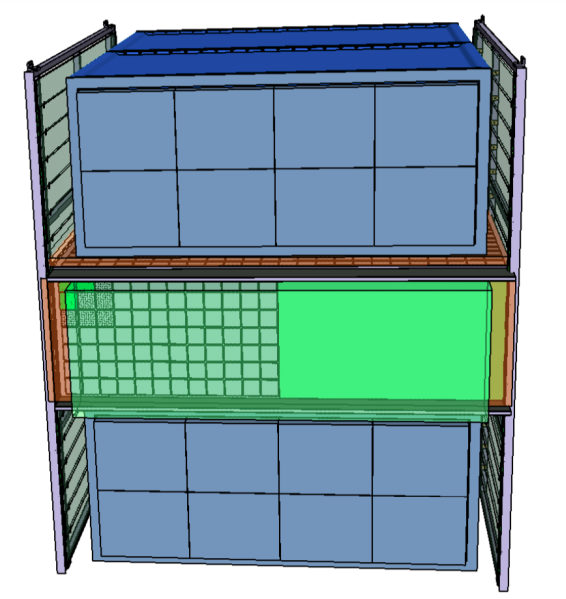
\includegraphics[width=0.5\linewidth]{HATPC_large}
  \caption{The upstream detectors of the upgraded ND280: HA--TPC (blue) and scintillator target (green). Beam is coming from the left. On the CAD the cathode dividing the drift volume and the Micromegas on the edge of the boxes can be seen.}
  \label{fig:up:tpc_large}
\end{figure}

\section{HA--TPC design}
\subsection{Requirements}
For the precise neutrino oscillation analysis, it is critical to meet the requirements of the existing TPCs and to study the possibilities of improvements. The momentum resolution of the current TPCs is ~10\% at the momentum around 1 GeV/c. It was driven by the accuracy of the neutrino energy reconstruction. The quasi--elastic reaction is assumed to compute the incoming neutrino energy from the outgoing lepton momentum. In this assumption, an initial nucleon stays at rest and is free. We are studying neutrino interactions with the nuclei where nucleons don't satisfy these conditions. Thus the reconstructed neutrino energy will be smeared because of nuclear effects. Fermi motion will be the dominating smearing effect. In the Oxygen and Carbon nucleon movement is characterized by the Fermi momentum $p_F\approx 200$ MeV/c. It will give $\approx$10\% uncertainty for the neutrino energy measurements. With the HA--TPCs, we are going to measure tracks with high angle w.r.t. the beam thus with lower momentum. Lower momentum will result in the larger track curvature and more precise reconstruction. Hence the same spatial resolution as in the current TPC is the minimum requirement for the new detectors. We are going to use the resistive Micromegas (MM) technology (\autoref{sec:up:res}) that will allow making the pads larger, but keep the spatial resolution unchanged or even slightly improve it. The spatial resolution of the current TPCs is at the level of 800 $\mu\text{m}$.

The other critical point for the ND280 performance is the dead material between subdetectors. The TPCs provide excellent tracking for the charged particles so it's strongly desired to detect all the particles that exit the scintillator towards the TPCs with minimal distortions. In the case of a massive field cage or a high Z material, several particles will lose the energy and suffer from multiple scattering making the precise measurements impossible. In the new TPCs, we are going to use a field cage made of a solid insulator laminated on a composite material. Thus the dead material between the scintillator target and the HA-TPC will be minimized. It's an important improvement as high--angle tracks are low energetic and even a small amount of material can cause track distortions. Also, the new field cage will maximize the fiducial volume of the detector.

A good energy resolution is essential for the separation of electrons and muons. As we are going to measure $\nu_e$ cross--sections while the $\nu_e$ contamination in the neutrino beam is at the level of 1\% the superior $e/\mu$ separation in the TPC is required. The current TPCs provide an 8\% energy resolution that results in 4$\sigma$ separation between electron and muon. The performance of the new detectors should be at least at the same level.

\subsection{Conceptual design}
The schematic view of the HA--TPC is presented in Figure~\ref{fig:up:tpc_s} and the main parameters are listed in \autoref{tbl:up:tpc_p}. The TPC will consist of a rectangular box divided into 2 parts by the high voltage cathode. The box serves as a gas vessel and a field cage (\autoref{sec:up:fc}). The maximum drift distance in each module is 90 cm. The same $\text{Ar:CF}_4\text{:iC}_4\text{H}_4$ gas mixture as in the existing TPC will be used. It will provide a drift velocity at the level of 7.8 $\text{cm/}\mu\text{s}$ resulting in a maximum drift time 11.5 $\mu$s. The electronics will sample the measurements every 40 ns and store in total 511 samples (20$\mu$s window). Thus tracks from the whole drift distance will be stored. The time window will cover the whole accelerator bunch which is distributed by Gauss with $\sigma=19$ ns. The field cage provides a uniform electric field with strength 275 V/cm inside the box. The high field uniformity is necessary for the uniform electron drift velocity. The latter is essential for the precise measurements of the track position along the drift distance. The signal from the drift electrons is amplified and read-out with the 16 Micromegas modules, 8 at each side. Each module has dimensions of 340$\times$410 $\text{cm}^2$ and is paved with 32$\times$36 pads 10$\times$11 $\text{mm}^2$ each. The pads are covered with the resistive foil that provides a charge spreading, improves the detector spatial resolution, and prevents Micromegas discharges (\autoref{sec:up:res}). The analog electrical signal from the pads is digitized with Front--End Cards (FEC), processed with Front--End Mezzanine cards (offset correction, zero-suppression, etc.), and then transferred to the ND280 global data acquisition system. The FEC and FEM cards are mounted on the TPC itself. The signal acquisition scheme is similar to the one we use in the existing TPCs.

\begin{table}
\begin{minipage}[!ht]{0.49\linewidth}
  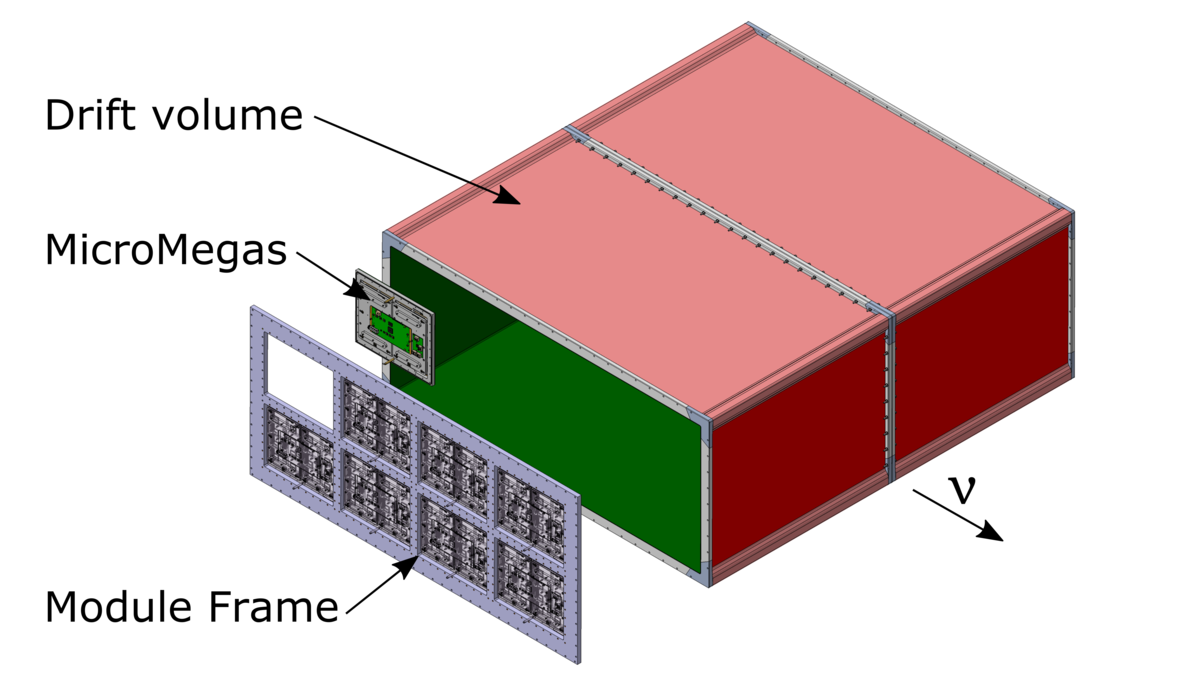
\includegraphics[width=\linewidth]{HATPC_scheme}
  \captionof{figure}{The schematic view of the new TPC}
  \label{fig:up:tpc_s}
\end{minipage}
\hfill
\begin{minipage}[!ht]{0.49\linewidth}
  \begin{tabular}{|c|c|}
    \hline
    Parameter             & Value \\
    \hline
    Overall x$\times$y$\times$z (m)   & 2.0$\times$0.8$\times$1.8 \\
    Drift distance (cm)               & 90 \\
    Magnetic Field (T)                & 0.2 \\
    Electric field (V/cm)             & 275 \\
    Gas $\text{Ar:CF}_4\text{:iC}_4\text{H}_4$ (\%)            & 95-3-2 \\
    Drift Velocity cm/$\mu$s          & 7.8 \\
    Transverse diffusion ($\mu$m/$\sqrt{\text{cm}}$) & 265 \\
    Micromegas gain                   & 1000 \\
    Micromegas dim. z$\times$y (mm)   & 340$\times$410 \\
    Pad z$\times$y (mm) & 10$\times$11 \\
    N pads                            & 36864 \\
    el. noise (ENC)                   & 800 \\
    S/N                               & 100 \\
    Sampling frequency (MHz)          & 25 \\
    N time samples                    & 511 \\
    \hline
  \end{tabular}
  \caption{Main parameters of the new TPC}
  \label{tbl:up:tpc_p}
\end{minipage}
\end{table}

\subsection{Field cage}
\label{sec:up:fc}
The requirements set for the field cage are to contain as little material as possible and use only low Z elements to minimize photon conversion and a charged particle scattering. At the same time, the box should be tight enough to hold the gas pressure without leakage, prevent atmospheric Oxygen and Nitrogen from entering the box, and contaminating the gas mixture. The walls of the field cage should be flat to prevent high voltage discharge. To meet the requirements mentioned above a composite material was chosen for the cage box. The composite materials are widely used in the industry. The TPC wall is going to consist of an Aramid honeycomb core and laminate skins on both sides of the core. In the inner part, the box will be covered with Kapton foil covered by Copper strips. It is the main field forming element of the structure.

The total thickness of the new field cage is 30 mm and its fraction to the radiation length is $d/X_0=1.7\%$. This value is improved comparing to the existing TPC. The old setup consists of two nested boxes 14 and 12 mm thick separated with a 68 mm gap. Also, heavier materials were used. The new structure minimizes the dead space between the HA--TPCs and scintillator targets by three times and suppresses the particle track distortions.

\subsection{Resistive Micromegas technology}
\label{sec:up:res}
The resistive bulk Micromegas technology is going to be used as a readout detector of the HA--TPCs. The TPC working principle is described in \autoref{sec:t2k:tpc} of \autoref{ch:T2K:general}. In short, the drift electrons are amplified with the high electric field between the micro--mesh and readout pads (\autoref{fig:up:res} left). The analog electrical signal is formed in the pads and further transported to the readout electronics. The bulk Micromegas~\cite{Giomataris2005} was proved to have excellent performance and long life--time in the existing experiments. The technique is laminating a woven mesh on a Printed Circuit Board (PCB) covered by a photoimageable film. This part is a sensitive detector. On top, the micromesh is put and fixed with an insulator above and below the mesh. The gap between the mesh and the PCB is the amplification region. The Micromegas technology minimizes the dead space on the detector plane and provides an excellent gain uniformity over the whole detector area. They have been operated in the experiments for a long period and the aging effect was found negligible.

\begin{figure}[!ht]
  \centering
  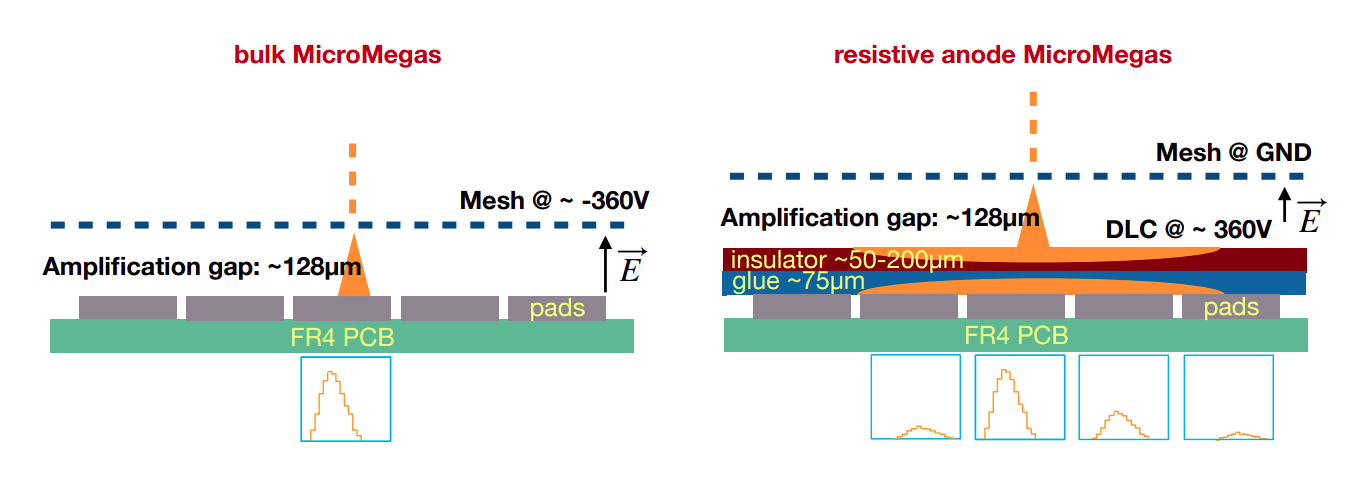
\includegraphics[width=0.95\linewidth]{mm_new}
  \caption{The schematic view of the bulk Micromegas operation without the resistive foil (left) and with resistive foil (right). The charge spreading due to the resistive foil is illustrated.}
  \label{fig:up:res}
\end{figure}

The resistive Micromegas is an upgrade for the existing technology. An insulator layer made from Kapton is glued to the pads. The Kapton layer is covered with a thin Diamond-Like-Carbon structure (DLC) (\autoref{fig:up:res} right). Such a design provides natural avalanche quenching. Thus the Micromegas discharge is prevented and there is no need for protection diodes in the front--end electronics. The resistive layer serves as a two dimensional RC network spreading the charge over the pads. For a point-like charge source the charge density versus the time $t$ and radius $r$ is described by the exponential law:
\begin{equation}
\rho(r,t)=\frac{RC}{2t}e^{-2r^2RC/\left(4t\right)}
\end{equation}

where $R$ and $C$ are resistivity and capacitance for unit area respectively. For example, giving the shaping time equal to 100 ns, resistivity equal to 400 $\text{k}\Omega/\square$, and glue thickness set to 75 $\mu\text{m}$ (controlling the capacity) the standard deviation of the charge spreading is expected to be 2.6 mm. Thus the spreading can be controlled with both resistivity and capacity. For example, for the larger spreading, the resistivity can be decreased or/and the thicker glue layer can be used (smaller capacity).

The effect of the charge spreading can improve the spatial resolution of the setup. If the electron cloud is close to the pad center and is smaller than the pad size. In the absence of the resistive foil, only one pad will register the signal. In such a case the spatial resolution will be limited by the pad size. However, with the charge spreading all the neighbor pads will register some signal. Even a simple barycenter measurement~\cite{Dixit2004} can improve the spatial resolution comparing to the traditional Micromegas. This improvement is the most significant at small drift distances when the electron cloud is compact and not has yet expanded with the transverse diffusion. In the ND280 TPCs, we observed a dramatic degradation of the resolution for the drift distances smaller than 200 mm because of this effect. The spectacular spatial resolution improvement down to 70 $\mu\text{m}$ with the resistive Micromegas was found for the International Linear Collider (ILC) TPC prototype~\cite{Attie2011}. For the case of the T2K, the resistive Micromegas allows using larger pads without any degradation of the detector performance.

\subsection{Electronics}
\label{sec:up:tpc_ele}
The architecture of the HA--TPC data acquisition system is schematically shown in \autoref{fig:up:tpc_ele_1}. The analog electric signal from the pads first goes to the Application Specific Integrated Circuit (ASIC)~\cite{Baron2007} called AFTER. They are used in the existing TPC and were proved to have low noise rate, high range of sampling frequency (up to 50 MHz), shaping time (100 ns $\div$ 2 $\mu$s) and gain (120 fC $\div$ 600 fC). Each ASIC collects information from 72 pads and provides only one analog output. The 511-cell deep circular buffer is used to store the signal from each pad. Together with sampling frequency, it sets the time window for signal acquisition. The nominal sampling time is 40 ns (25 MHz) that gives an acquisition window nearly twice larger than the maximum drift time. 8 ASICs are mounted on the Front End Card chip (FEC) that performs the signal digitizing. Two FECs are inserted directly at the Micromegas back and connected to the pads with pitch connectors. Front End Mezzanine Card (FEM) is mounted on top of each two FECs and synchronizes signal digitization with a master clock. At FEM all the data from AFTER chips are collected and zero suppression is applied. All the electronics mentioned above are located inside the magnet. From the FEM the signal is transferred outside the magnet with the optical fiber. The CADs of the electronics that are mounted on the Micromegas inside the basket is provided in \autoref{fig:up:tpc_ele_2}. The cards' temperature is maintained with the water cooling system.


\begin{figure}[!ht]
  \centering
  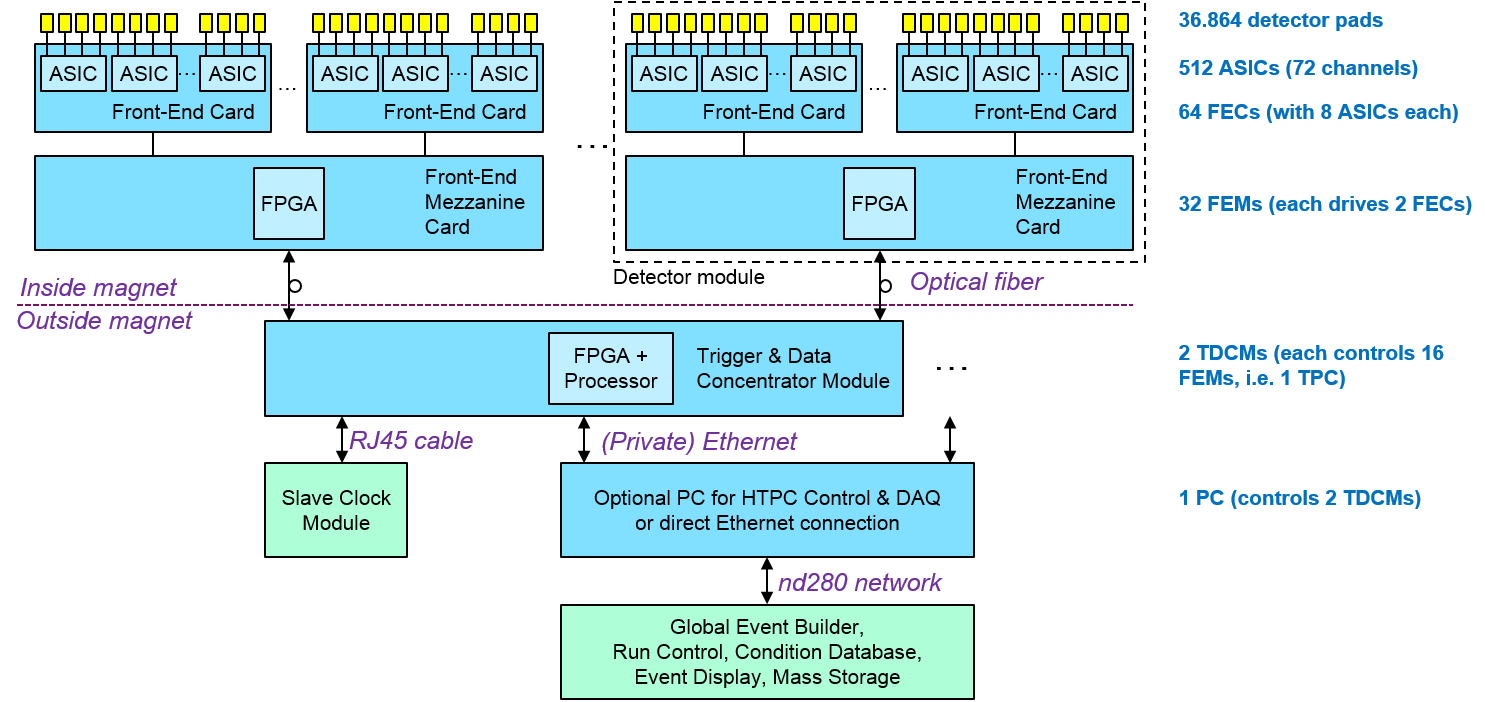
\includegraphics[width=0.8\linewidth]{tpc_ele}
  \caption{Scheme of the TPC electronics system.}
  \label{fig:up:tpc_ele_1}
\end{figure}

The digitized and pre-processed data is transferred with the optical fiber to the Trigger and Data Concentrator Module (TDCM). Each unit reads data from 16 Micromegas and provide timing synchronization and trigger signals to the FEMs. The TDCMs communicate with the global ND280 data acquisition system with a standard Gigabit Ethernet link.

\begin{figure}[!ht]
  \centering
  \begin{minipage}{0.49\linewidth}
    \centering
    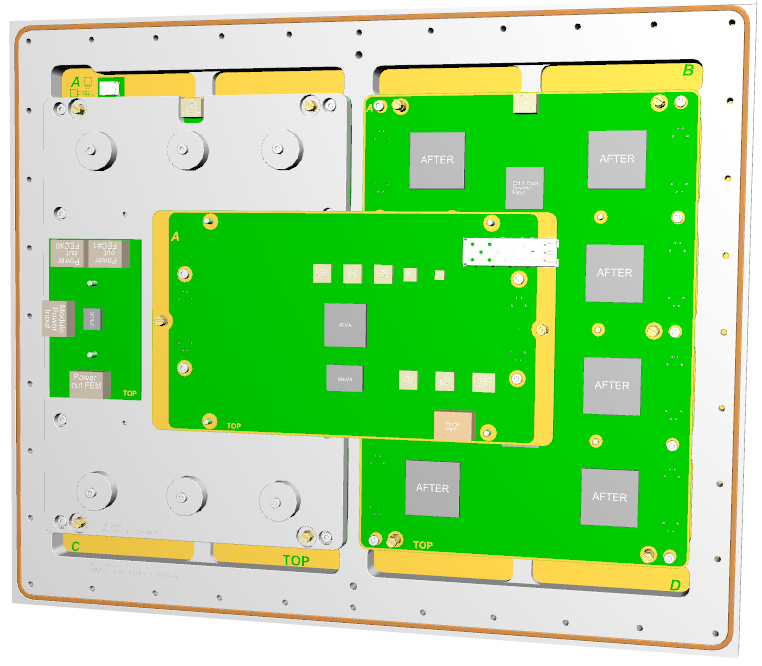
\includegraphics[width=\linewidth]{MM_ele_1} \\ (a)
  \end{minipage}
  \begin{minipage}{0.49\linewidth}
    \centering
    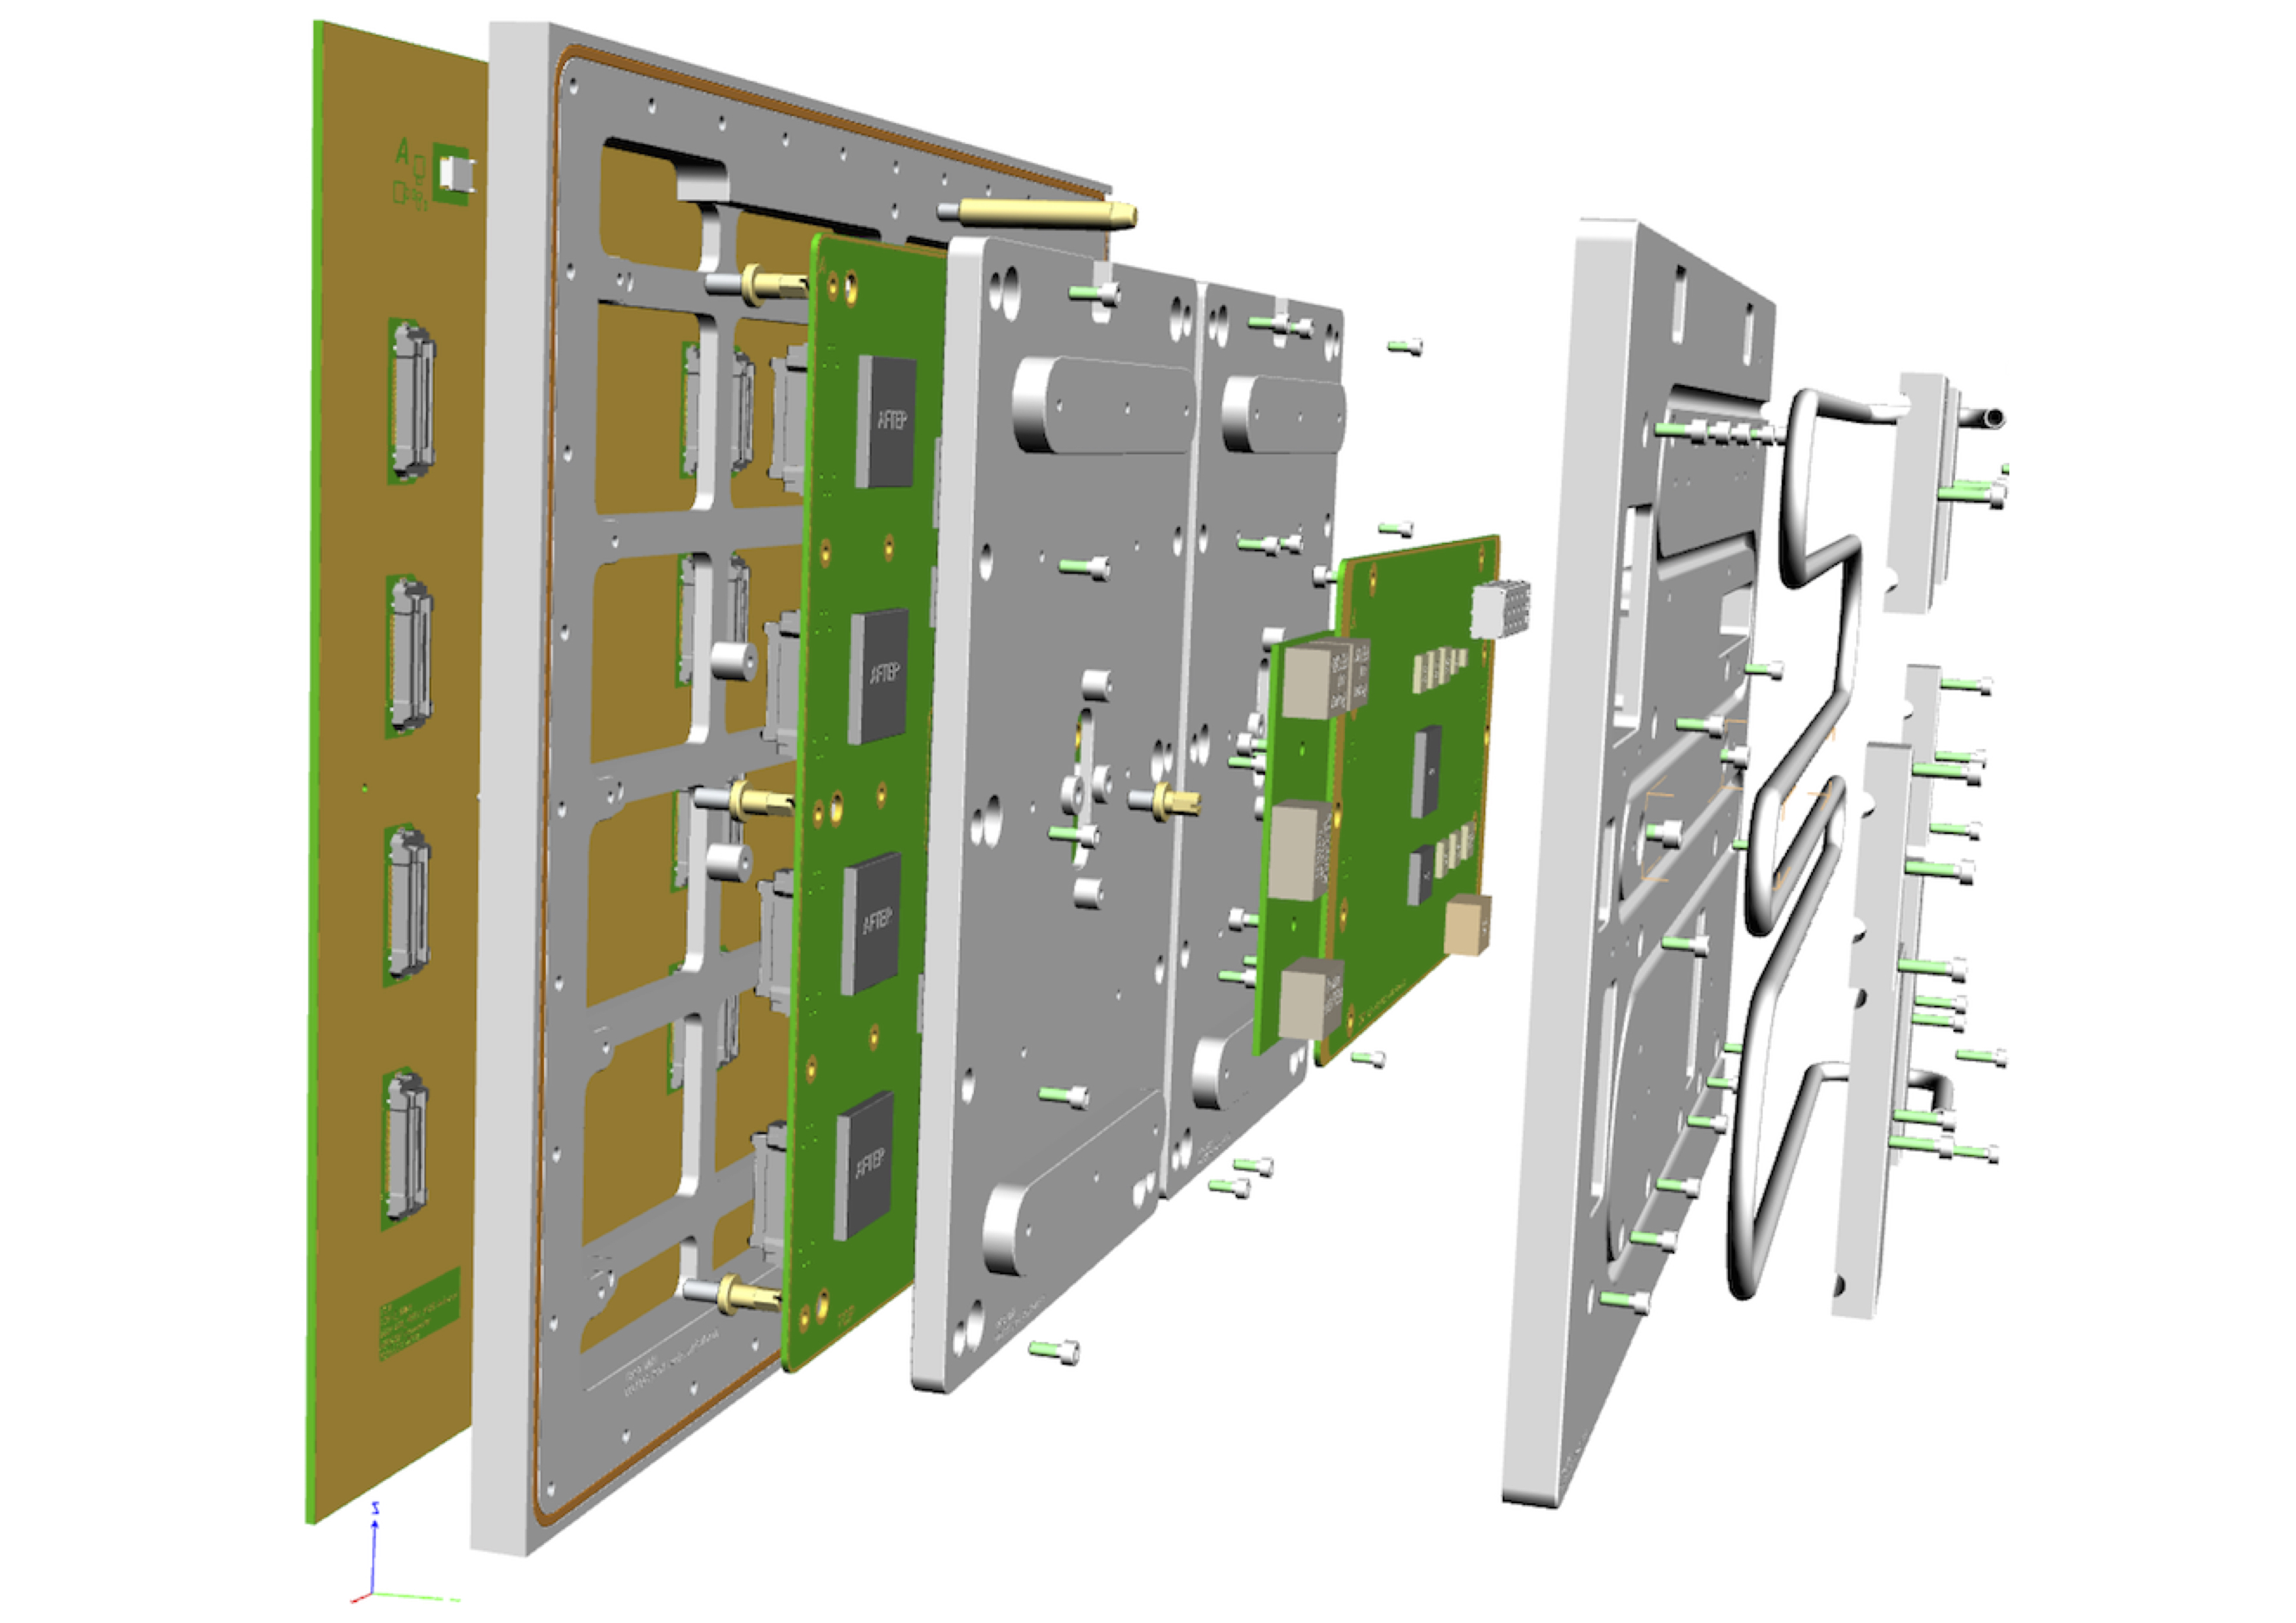
\includegraphics[width=\linewidth]{MM_ele_2} \\ (b)
  \end{minipage}
  \caption{The CAD of the HA--TPC electronics mounted on the Micromegas without the cooling system (a) and sectional view of the whole setup (b).}
  \label{fig:up:tpc_ele_2}
\end{figure}

\section{Prototype tests}
An improved spatial resolution is going to be achieved with the new TPC with a resistive anode. At the same moment, the energy resolution should not decrease as it's critical for the T2K $\nu_e$ measurements. Few detector prototypes were built and tested. The main goals of the tests are to test the detector production technology, to find the optimal hardware parameters and to estimate the spatial and energy resolution of the future detector.

\subsection{Cosmic test}
\label{sec:up:saclay}
The Micromegas prototype was produced for the test with the beam of charged particles at CERN beam test area. Before that, it was tested at the test bench in Saclay. The primary goal of the detector test was to figure out that the whole detector plane was operating as expected, the detector response is uniform and the Micromegas was not damaged.

The scheme and the photo of the setup are shown in \autoref{fig:tpc:photo_saclay}. The field cage with a 15 cm drift region was used for the test setup. It was filled with Argon (95\%) and Isobutane(5\%). The uniform electric field was maintained with the strips that you can see in \autoref{fig:tpc:photo_saclay} (b). The drift field was set to 183 V/cm. The resistive Micromegas was mounted on the side of the field cage. The size of the module was 36$\times$34 $\text{cm}^2$ and it was paved with 36$\times$48 pads 0.98$\times$0.70 $\text{cm}^2$ each. The same PCB as in the existing TPC was used.

The RC feature was implemented with a 200 $\mu\text{m}$ insulator layer (capacitance) and a 50 $\mu\text{m}$ Kapton with a thin Diamond-Like-Carbon layer (DLC) (resistivity). The resistivity value was set to 2.5 $\text{M}\Omega/\square$. The side pads are partly covered with a frame that is fixing the mesh and providing the grounding of the DLC. Thus the first and the last row/column are excluded from all the analysis as they are known to measure less charge than the other pads. The Micromegas voltage was varied for different samples during the data taking from 350 V up to 390 V. The front--end electronics were mounted on the outer side of the Micromegas and could be seen in \autoref{fig:tpc:photo_saclay} (c).

\begin{figure}
  \begin{minipage}{0,33\linewidth}
    \centering
    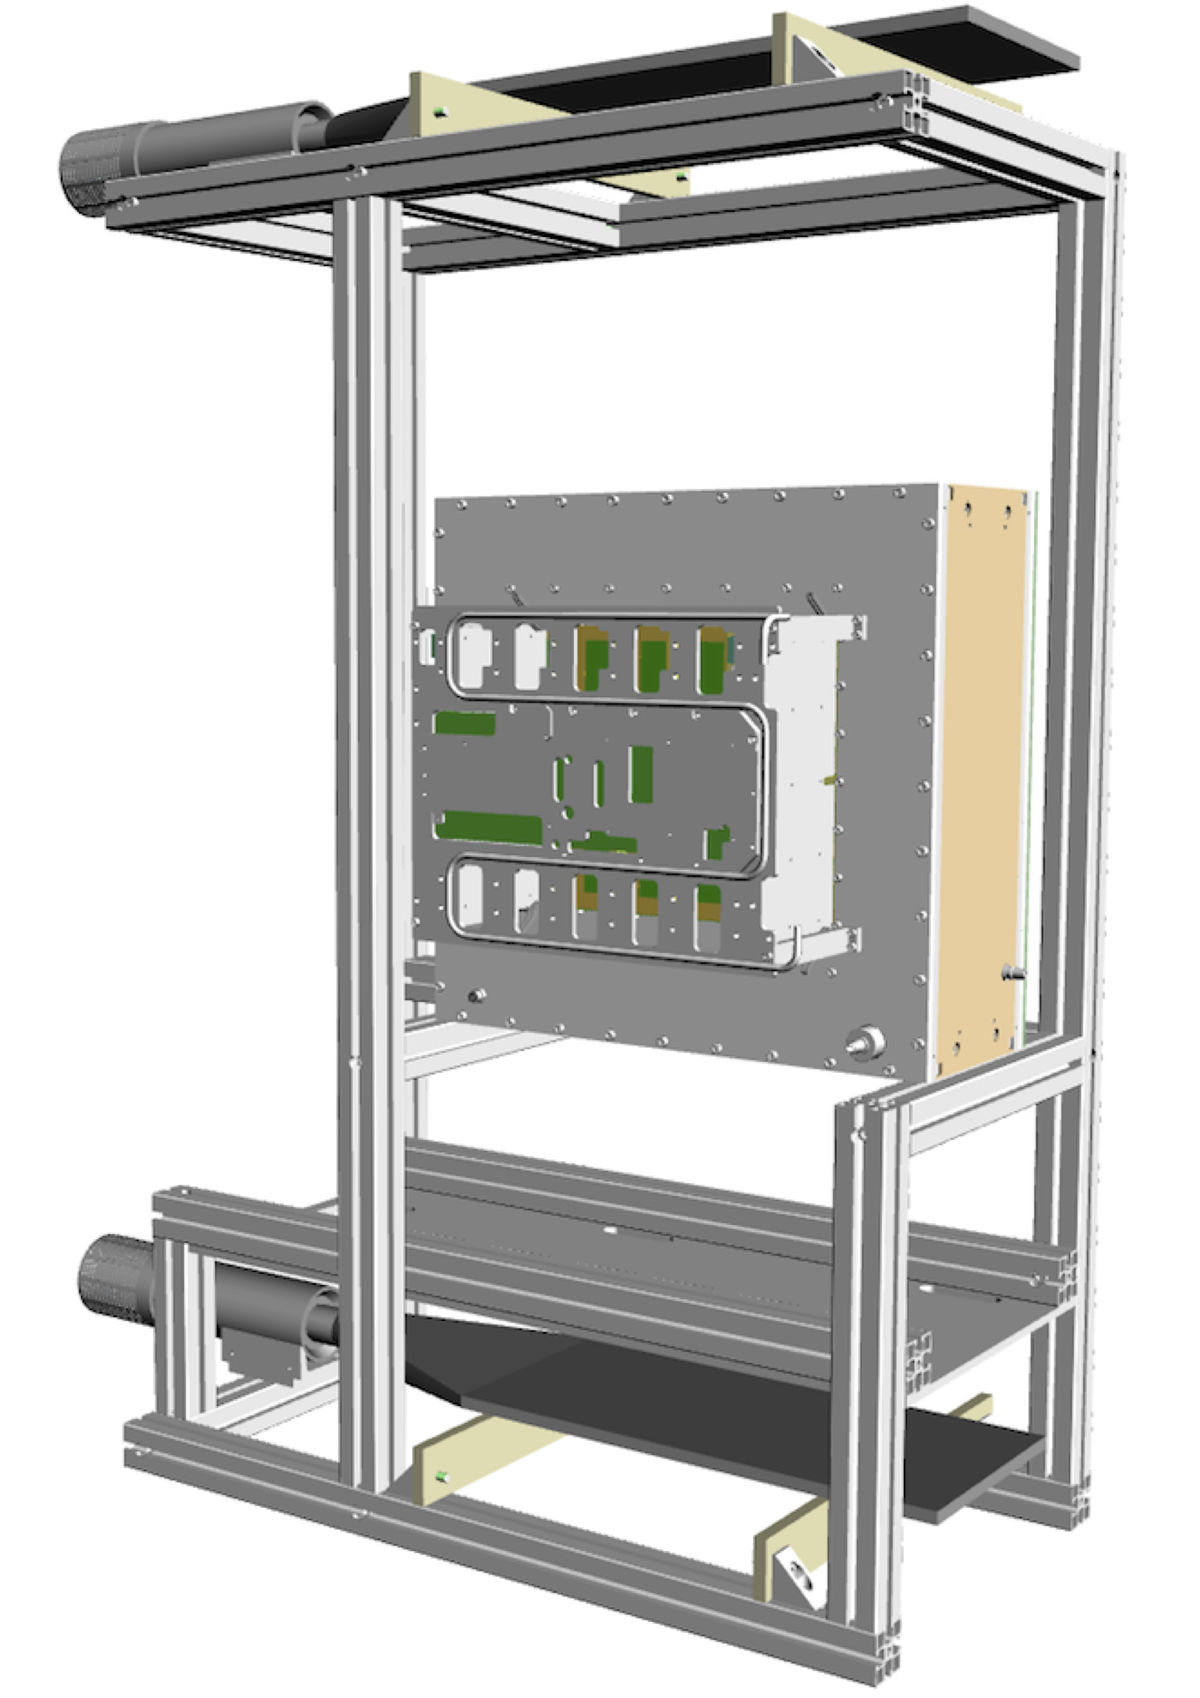
\includegraphics[width=0.5\linewidth]{Saclay_test_bench} \\ (a)
  \end{minipage}
  \begin{minipage}{0,33\linewidth}
    \centering
    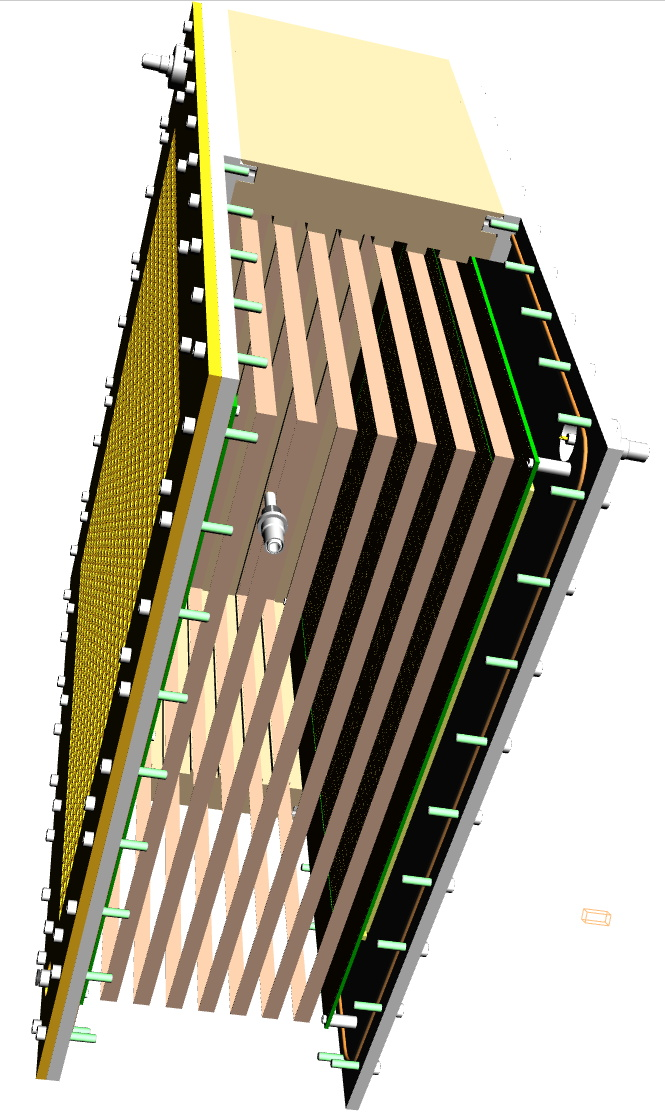
\includegraphics[width=0.5\linewidth]{testbenchTPC} \\ (b)
  \end{minipage}
  \begin{minipage}{0.33\linewidth}
    \centering
    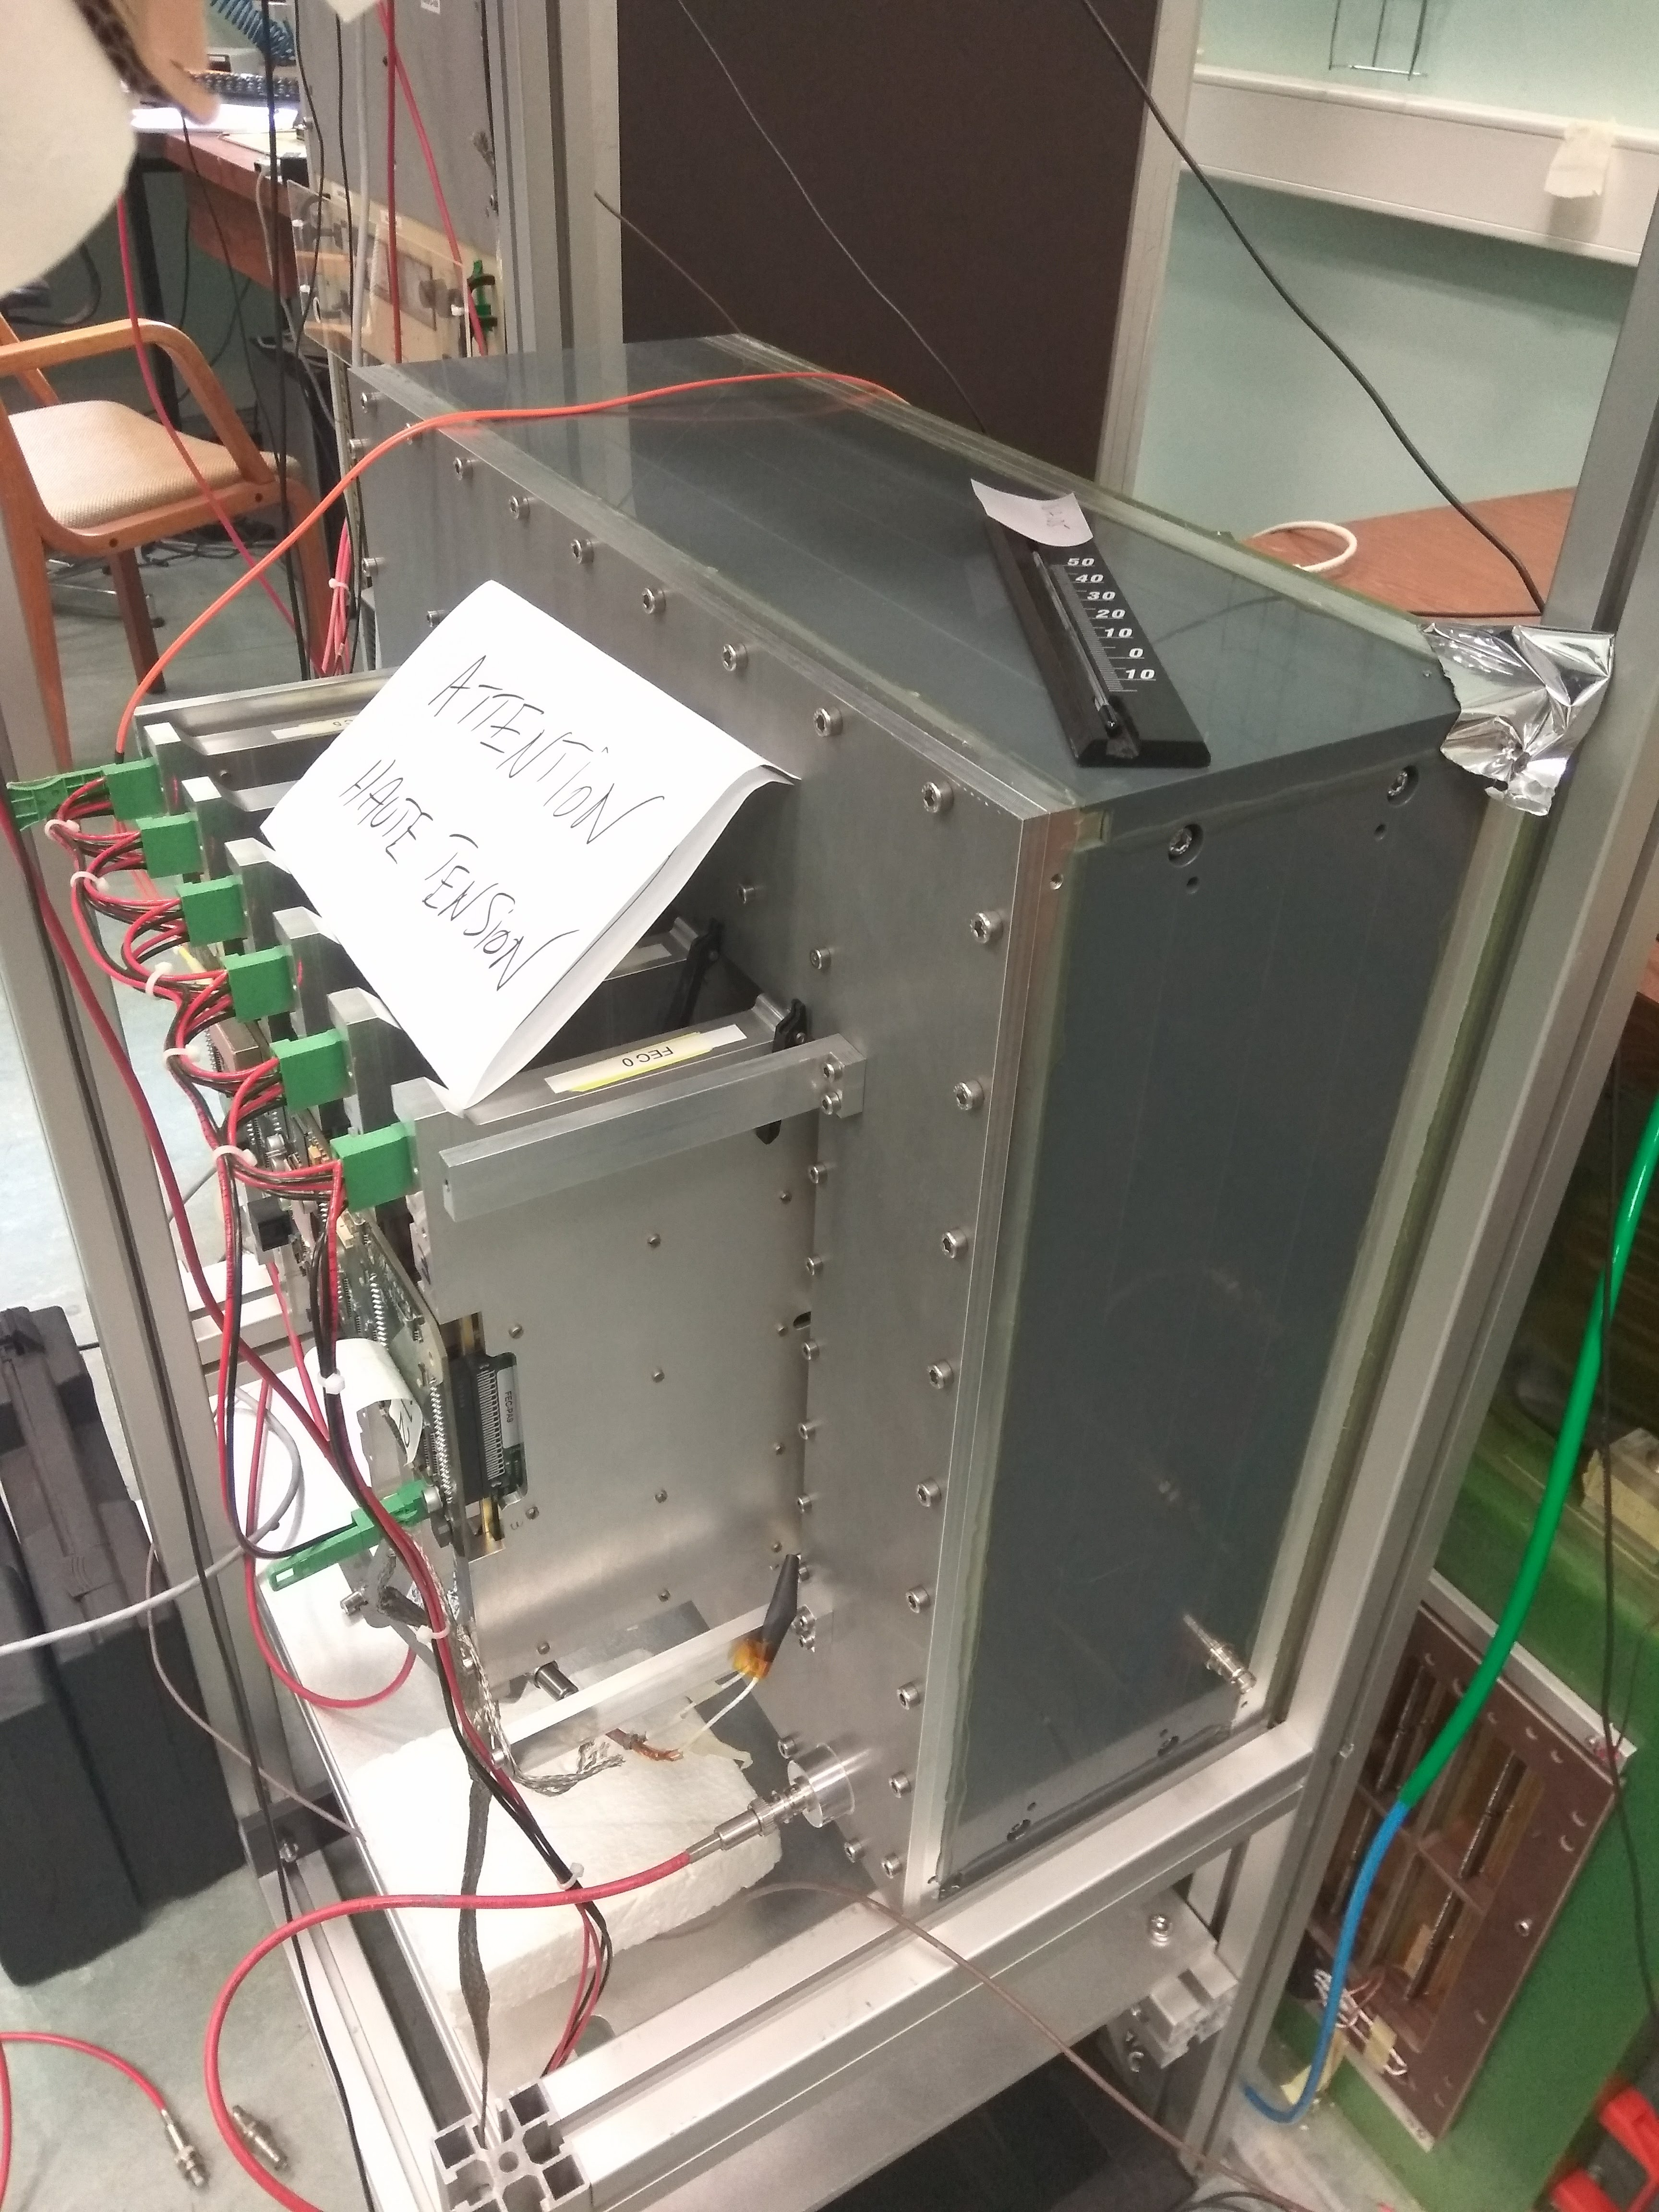
\includegraphics[width=0.5\linewidth]{tpc_saclay_ph} \\ (c)
  \end{minipage}
  \caption{TPC test bench in Saclay. (a) a CAD model of the whole test bench with the scintillator bars above and behind the detector as a trigger. (b) the CAD model of the field cage. (c) a photo of the test bench during the data taking.}
  \label{fig:tpc:photo_saclay}
\end{figure}

The data was taken with the cosmic rays and the X--ray radioactive source (${}^{55}\text{Fe}$). The trigger system for the cosmic muons was built around the setup. On the \autoref{fig:tpc:photo_saclay} (a) two scintillator planes above and below the detector are shown in dark gray. The planes are readout with photomultipliers and the coincidence of signal in two planes serves as a trigger for the through-going cosmic ray. From the ${}^{55}\text{Fe}$ source, we expect continuous decays, so we can sample the data nearly at any time. The pulse generator was used as a trigger for this sample.

As at any other detector, we expected to see a certain level of noise in our measurements. The noise level was measured for each channel independently. The pulse generator was used to sample the data from each pad. As we expected no signal in the pad the measured value should be caused by the noise and suppressed in future measurements. As the noise is a subject of fluctuation its value was measured for a continuous period. The measured values were fit with the Gaussian distribution and the mean and sigma characteristics were extracted from the fit. The mean value was going to be subtracted from every measurement done with this particular pad. The sigma value was used to treat the measured amplitude as a signal or a noise. If the amplitude was different from the mean value by more then four sigmas the measurement would be recorded. The procedure described above is called ``zero--suppression''. It is usually quantified with the value of standard deviations used to divide signal and noise, e.g. $4\sigma$ or $5\sigma$ zero--suppression.

The examples of the event displays are shown in \autoref{fig:tpc:saclay_ed}. As the gain supposed to be uniform over the whole Micromegas, we expect a uniform measured charge. I analyzed the hit map with merging the information from all the cosmic tracks together. The detector response was found uniform, thus the data from the prototype may be used for the further precise analysis.
% The hit map obtained with the cosmic rays is shown in \autoref{fig:tpc:hitmap_saclay}.

\begin{figure}[!ht]
  \centering
  \begin{minipage}{0.49\linewidth}
  \centering
    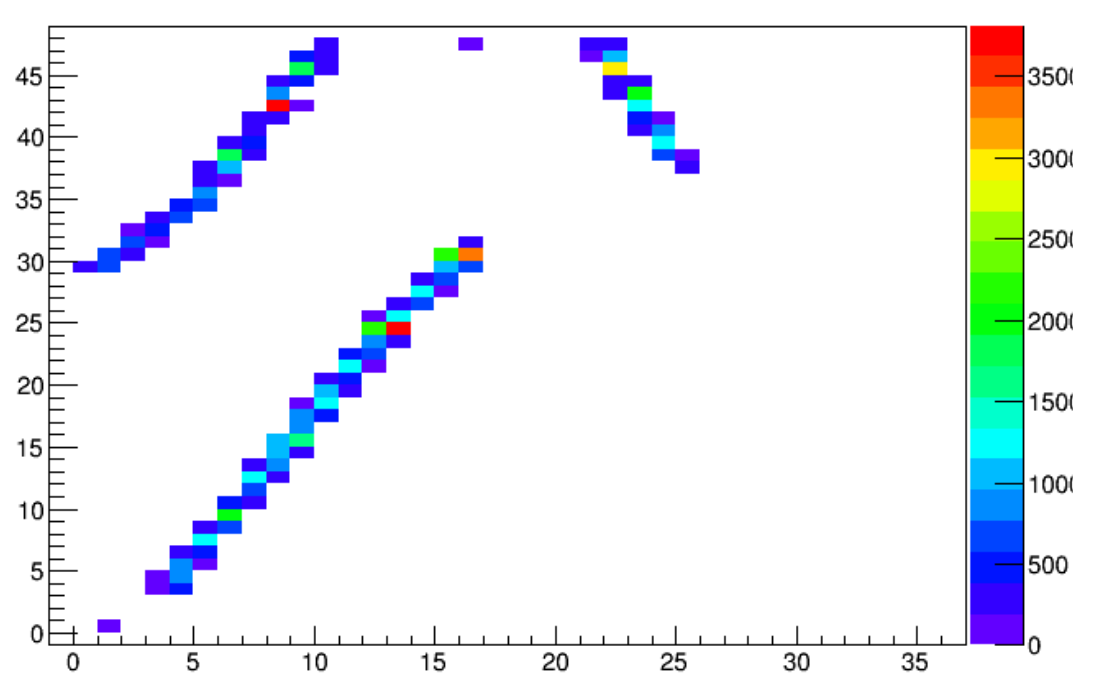
\includegraphics[width=0.8\linewidth]{saclay_ed_drift} \\ (a)
  \end{minipage}
  \begin{minipage}{0.49\linewidth}
  \centering
    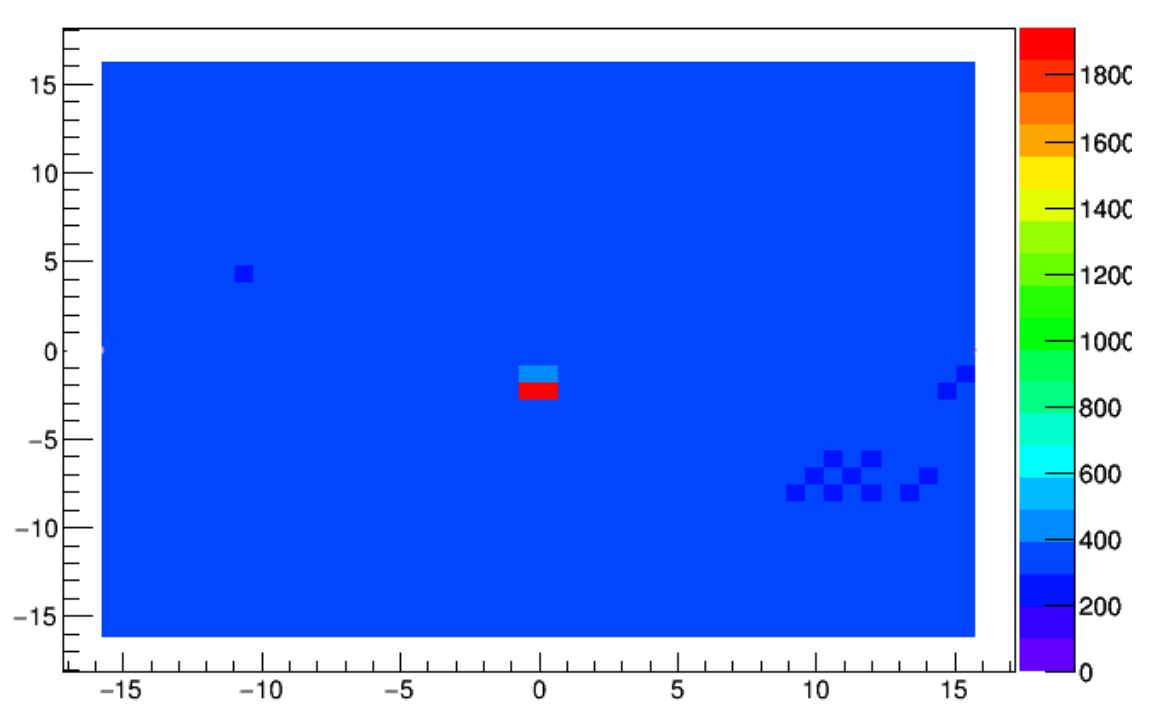
\includegraphics[width=0.8\linewidth]{saclay_source.png} \\ (b)
  \end{minipage}
  \caption{Events observed in the TPC prototype during the test in Saclay. (a) cosmic ray and (b) an X--ray detection from ${}^{55}\text{Fe}$ source.}
  \label{fig:tpc:saclay_ed}
\end{figure}

% \begin{figure}[!ht]
%   \centering
%   \begin{minipage}{0.49\linewidth}
%   \centering
%     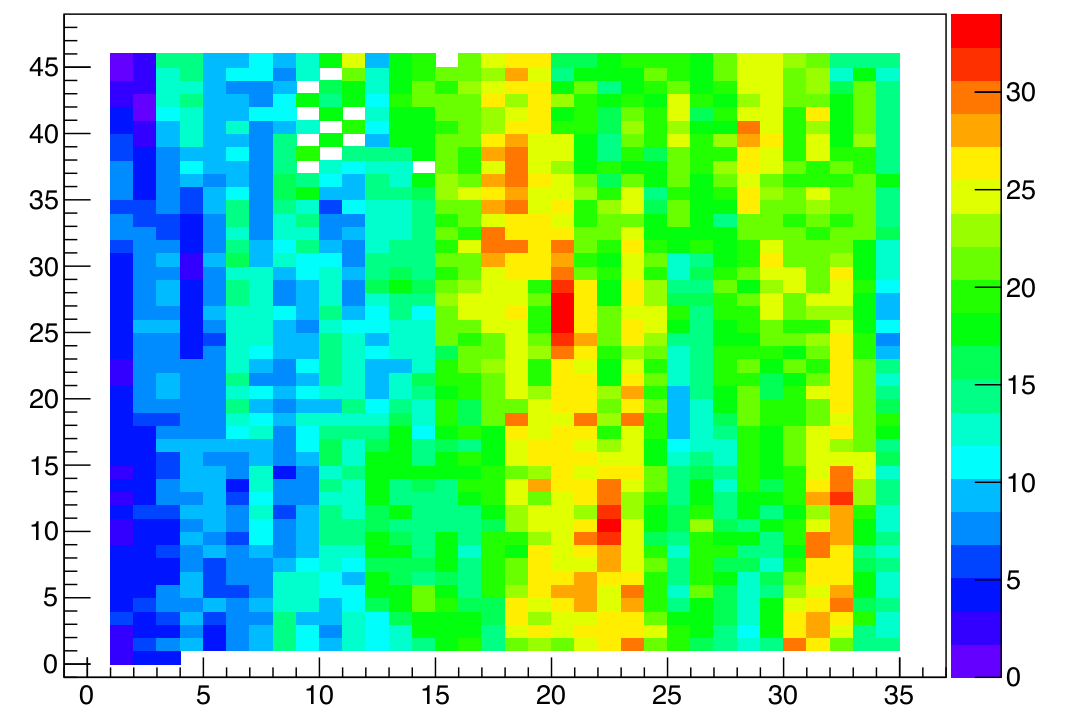
\includegraphics[width=0.8\linewidth]{saclay_hitmap} \\ (a)
%   \end{minipage}
%   \begin{minipage}{0.49\linewidth}
%   \centering
%     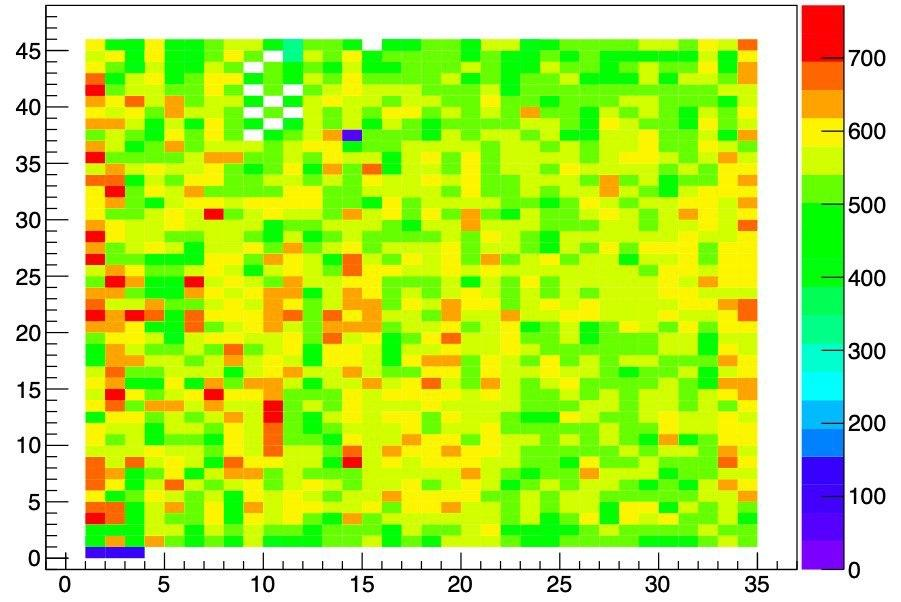
\includegraphics[width=0.8\linewidth]{saclay_hitmap_norm} \\ (b)
%   \end{minipage}
%   \caption{Hit maps observed in the TPC prototype during the test in Saclay. (a) how many times the particular pad was hit and (b) the average charge measured per a hit.}
%   \label{fig:tpc:hitmap_saclay}
% \end{figure}

At the hit maps, a cluster of the missed pads was observed at the top left part of the Micromegas. It was found that the problem was in the electronic connection in the readout system, but not in the Micromegas itself.

With the collected data I estimated the energy resolution of the detector with both cosmic rays and ${}^{55}$Fe source with a truncated mean technique (\autoref{sec:tpc:tpc_dedx}). The distribution of the dE/dx for cosmic tracks is shown in \autoref{fig:tpc:saclay_charge} and gives a 20\% energy resolution. The resolution measurement with cosmic rays is not precise. The energy loss depends on the muon energy. The dE/dx measurements from tracks are made for all the cosmic tracks in a whole spectrum. The obtained value is an upper limit and more precise measurements will be done during the beamtest. The analyses of the ${}^{55}$Fe events is more precise as the isotope is a monoenergetic source of 5.9 keV photons. The resolution for the 5.9 keV line was measured at a level of 7.3\% that is comparable with the performance of the existing detectors~\cite{Abgrall2011}.

The charge spreading in the Micromegas is the main feature in the prototype. The spreading needs to be measured and prove to be working. As we are working with the vertical cosmic tracks the number of triggered pads in a row is a good metric to quantify the charge sharing between the pads. We will call this metric ``pad multiplicity''. Without the resistive foil, with a small drift distance, we expect to have one pad illuminated if the track goes over the pad center and two pads if the track goes over the pad border. The pad multiplicity for the vertical cosmic rays going through the TPC prototype is shown in \autoref{fig:tpc:savlay:mult}. Clusters with two pads are dominating. We also have some clusters with more than two pads in a row that is completely impossible in the absence of the resistive layer. Thus we have a clear indication that the RC network is working. Though there are many pads with only one pad in a row. It may be caused by the low ionization by the cosmic muon or by not sufficient charge spreading in the Micromegas. The beam test will provide more accurate result. The resistivity of the Micromegas can be tuned according to obtained results.

\begin{figure}[!ht]
  \centering
  \begin{minipage}{0.45\linewidth}
    \centering
    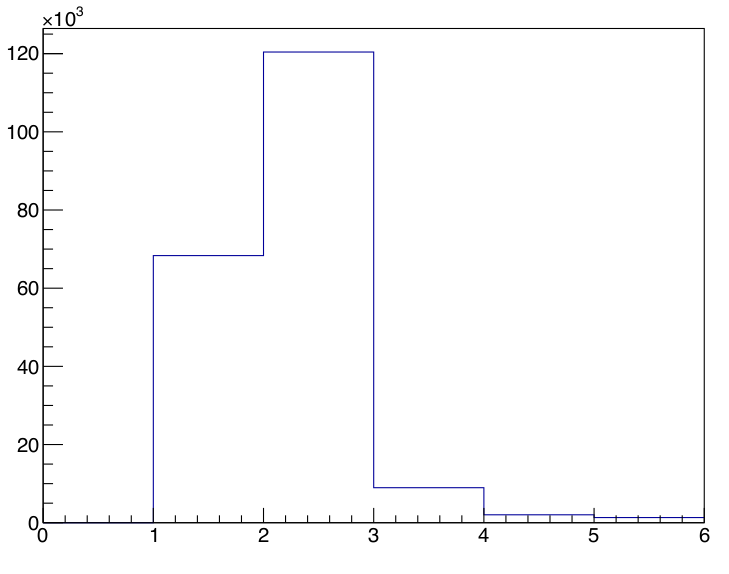
\includegraphics[width=\linewidth]{saclay_multi}
    \caption{The number of pads in a row for the vertical cosmic track (pad multiplicity) in the TPC prototype at Saclay.}
    \label{fig:tpc:savlay:mult}
  \end{minipage}
  \begin{minipage}{0.09\linewidth}
    \hspace{\linewidth}
  \end{minipage}
  \begin{minipage}{0.45\linewidth}
    \centering
    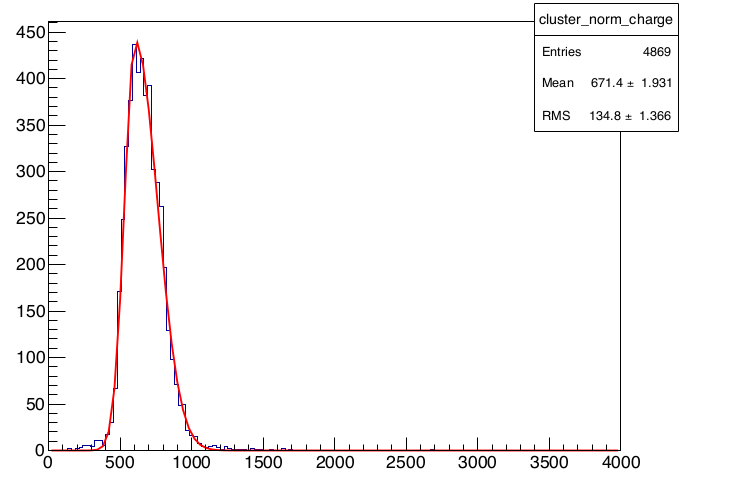
\includegraphics[width=\linewidth]{saclay_trunc}
    \caption{The distribution of the average charge per cluster after the truncation fit with Gaussian function.}
    \label{fig:tpc:saclay_charge}
  \end{minipage}
\end{figure}

To sum up, the detector was tested at the test bench with cosmic rays and ${}^{55}\text{Fe}$ source. The measured energy resolution for the isotope is similar to the performance of the existing TPCs. The charge spreading over pads was proved to be working. After these preliminary measurements detector will be tested at the beam of charged particles.

\subsection{CERN beamtest}
\label{sec:up:tpc:cern}
The Micromegas module tested with the cosmic rays in Saclay was further studied in CERN with the charged particle beam from the accelerator beamline.

\subsubsection{Setup}
The detector was mounted in the former HARP TPC field cage~\cite{Prior2003}. The HARP experiment was conducted in the early 2000s and was aimed at precise measurements of the hadron production on various solid and liquid targets. The high tracking performance was obtained with the HARP field cage. It is a 2 m long and 0.8 m diameter cylindrical volume that provides 1.5 m drift region. In our test setup, the cathode and Micromegas were mounted on the opposite edges of the cylinder and cathode set at 25 kV providing a drift field of 167 V/cm. A ${}^{55}\text{Fe}$ source was mounted on the cathode plane for the MM gain measurements. The gas mixture of $\text{Ar:CF}_4\text{:iC}_4\text{H}_{10}$ (95:3:2) was used to fill the gas volume. It is the same mixture that has been used in the ND280 TPCs. The electronics were the same that had been developed for the T2K TPCs. No magnetic field was used in this test. The photo of the setup is shown in \autoref{fig:cern:cern_ph}.

\begin{figure}[!ht]
  \centering
  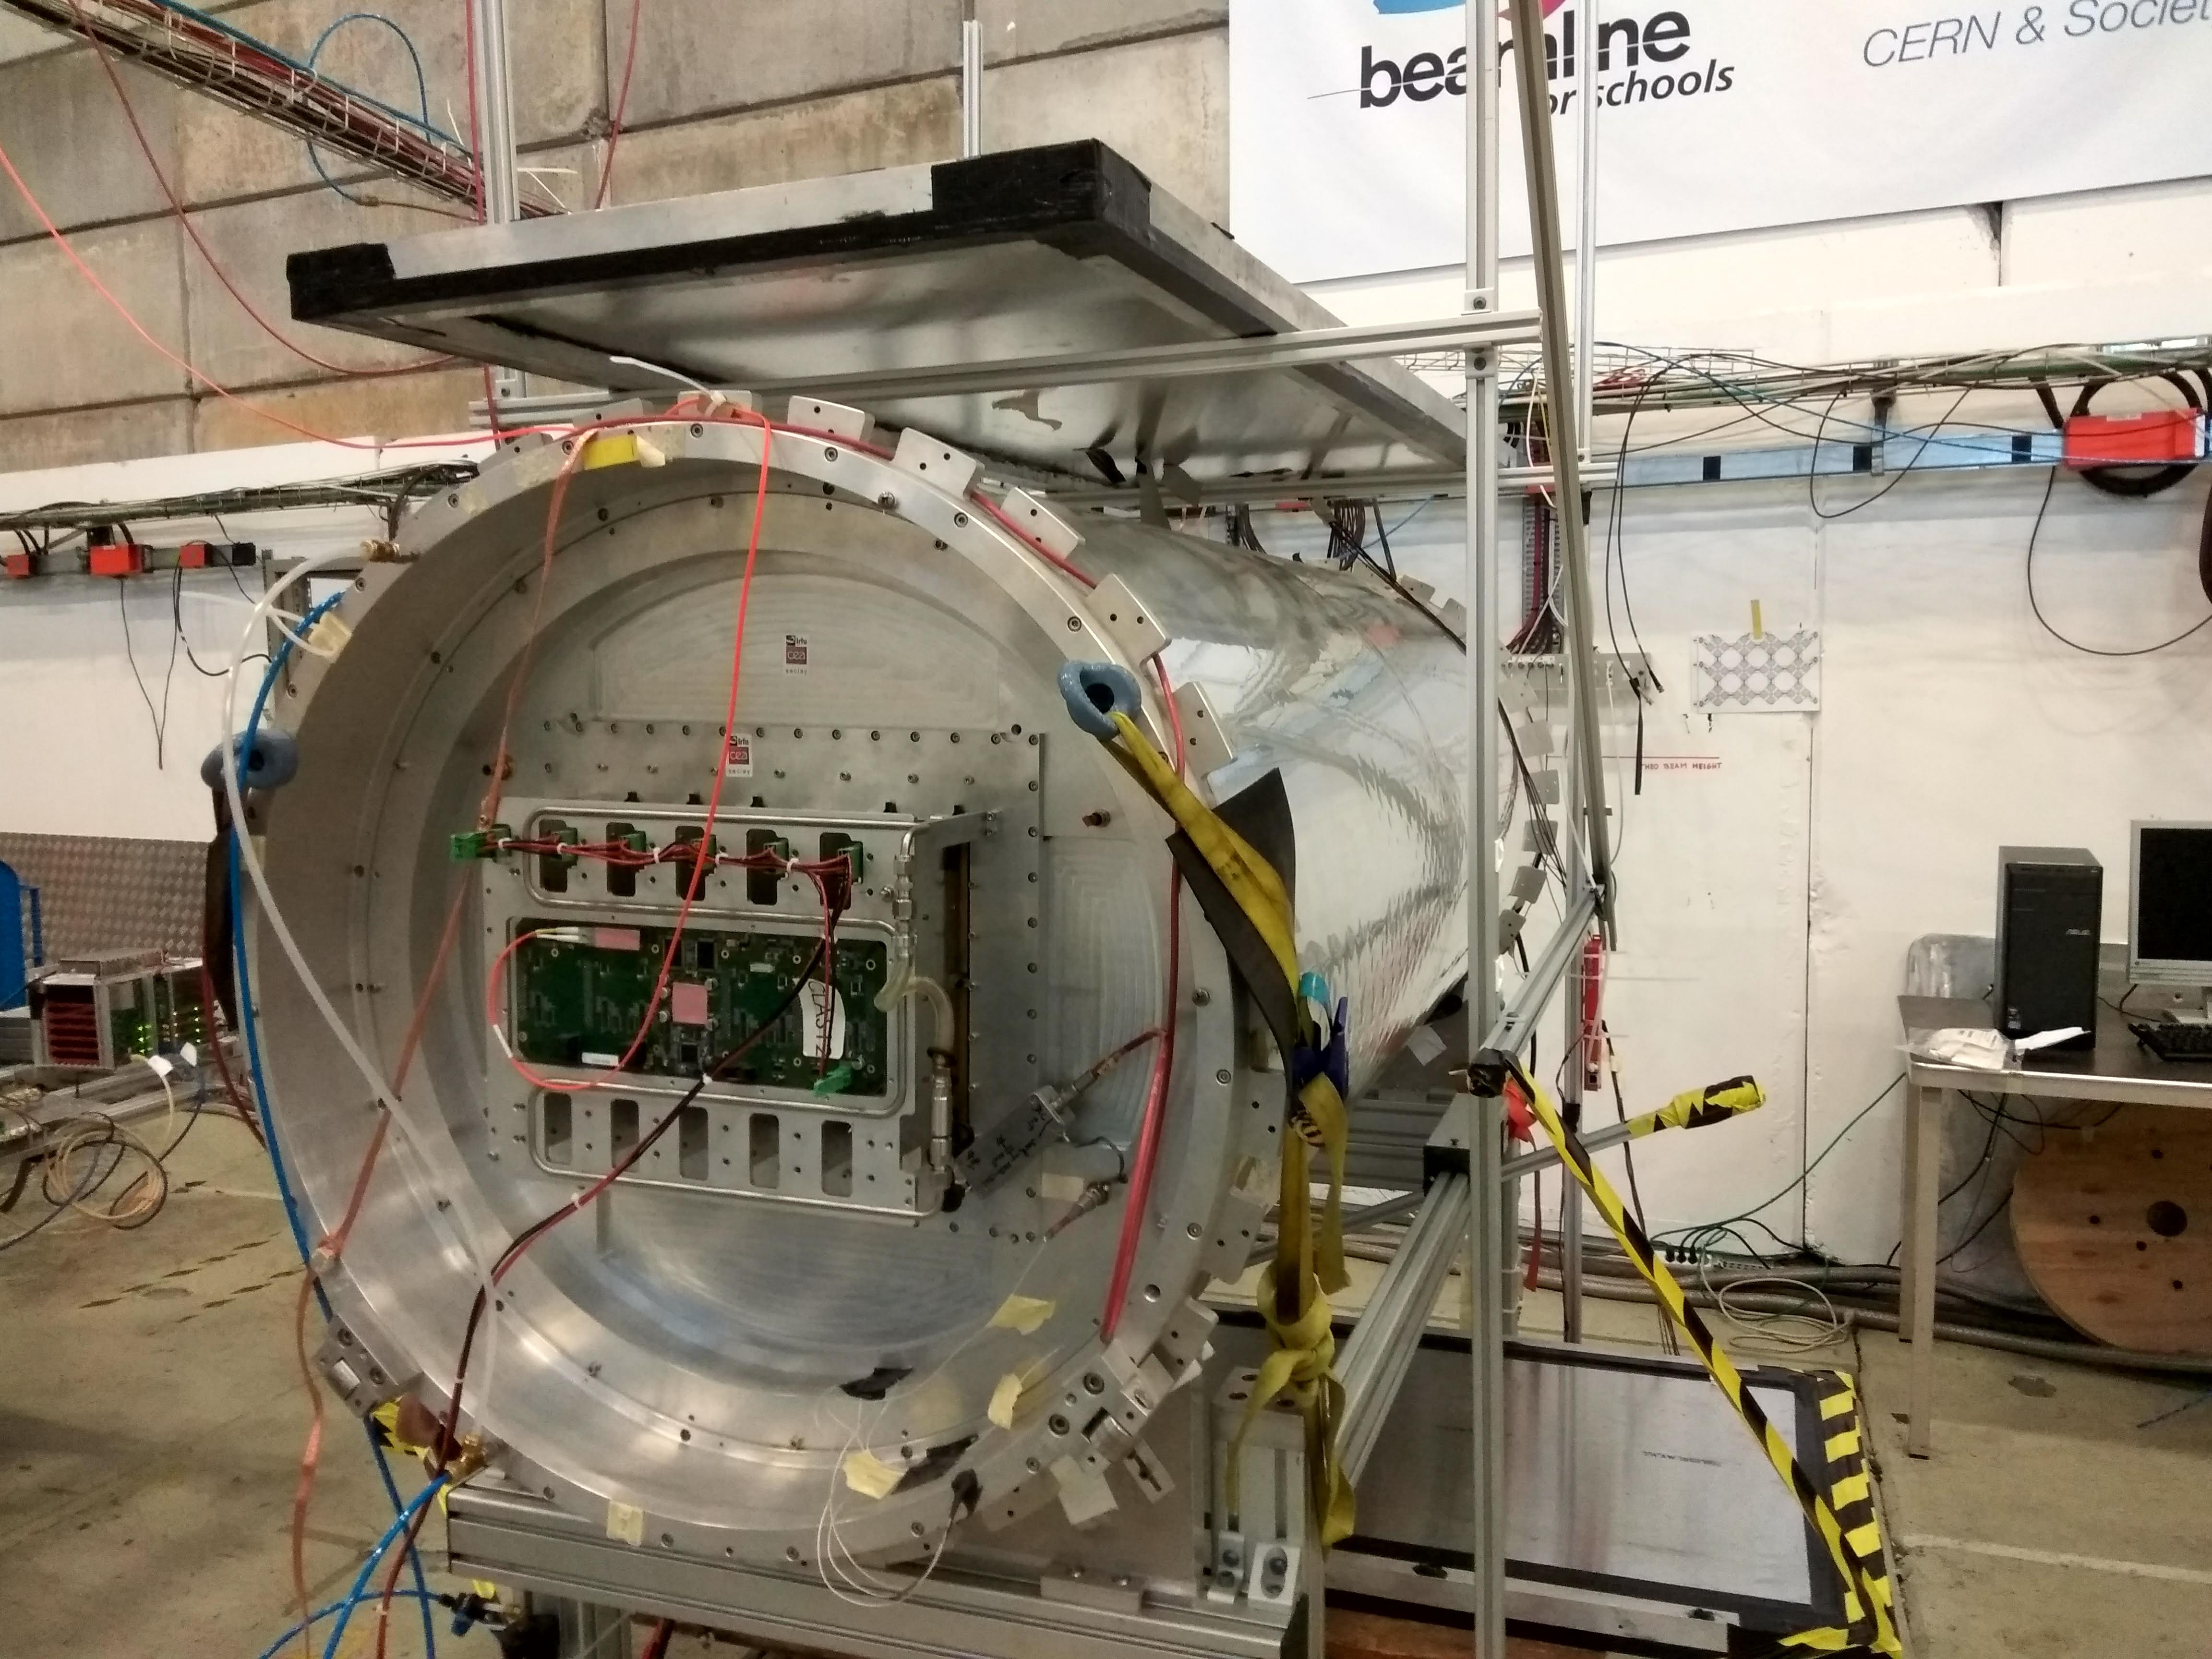
\includegraphics[width=0.7\linewidth]{cern_tpc_ph}
  \caption{The photo of the TPC prototype installed at the CERN beamline. The Micromegas are installed in the closes end cap of the cylinder field cage. The scintillator planes for the cosmic trigger are put above and below the TPC.}
  \label{fig:cern:cern_ph}
\end{figure}

CERN T9 beamline was used for the charged particle source. It is based on the proton synchrotron (PS) and was operated in the ``hadron enriched mode'' with a copper target. The beam polarity, momentum and focus point can be adjusted by tuning of the beamline magnets.
At the energies below 1 GeV the beam is mostly electron/positron, while above this energy it is mostly pions. The proton contribution is roughly one third of all the particles. These particles are important for the TPC tests as all of them can be produced with the neutrino interactions in ND280. The type of particles in the particular data sample is determined with the trigger system configuration. The scheme of the trigger system is shown in \autoref{fig:cern:trigger}.  For example, the Cherenkov detectors signals (C1, C2)  will explicitly indicate the electron or a positron, while for pion or a proton there should be no signal in these detectors. Pions and protons were separated with the time difference between the signal in the scintillator detectors (S1, S2, S3). Thus the beam data is divided into electron, proton and pion samples with the appropriate trigger consequence used. We expect the particles of certain type to dominate in each sample.

\begin{figure}[!ht]
   \centering
   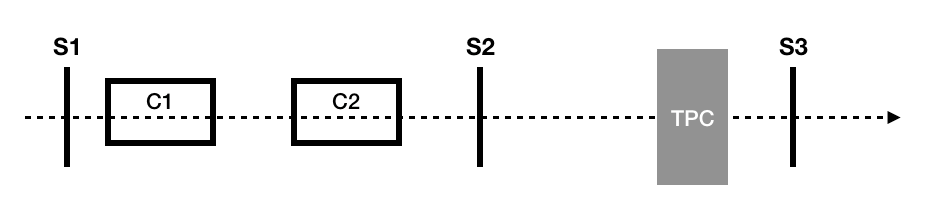
\includegraphics[width=0.6\linewidth]{cern_trigger}
   \caption{The scheme of the trigger system for the TPC prototype test at CERN beamline. The system consists of two Cherenkov detectors (C1, C2) and three scintillator detectors (S1, S2, S3).}
   \label{fig:cern:trigger}
 \end{figure}

The data were taken with three trigger activation schemes: electron, pion and proton and with three drift distances 10, 30, and 80 cm. During these scans, the Micromegas was operated with a voltage of 340 V, the electronics sampling and peaking time were set to 80 ns and 600 ns respectively. In addition, with the beamline and trigger set to 1 GeV/c pion selection, the MM voltage scan was performed. Samples with high voltage from 330 V up to 380 V with 10 V steps were taken. During the whole data taking, cosmic rays were also recorded. For this purpose, two scintillators panels were put above and below the field cage and served as a trigger. The signal readout from the panels was done with wavelength shifting fibers (WLS) and multi-pixel photon counters (MPPC). The cosmic trigger can be activated only outside of the beam window time. The signal from ${}^{55}\text{Fe}$ source was also collected. We expected a couple of source events for the drift time at a distance of 1.5 m (whole detector), so no additional trigger was set. We would be able to see enough source events in the samples with beam or cosmic tracks.

After the trigger arrives each pad is open for data recording with 511 time bins. Most of the time, the sampling of 80 ns was used. That gives us a time window 1.5 times larger than the expected drift time for the whole TPC length. The $4\sigma$ zero suppression was used with a similar technique that was described in the Saclay test. The signal in the particular pad is stored only if the maximum amplitude was higher than the mean noise by more than 4 standard deviations. The examples of the waveforms are shown in \autoref{fig:tpc:cern_wf}. There are few options for the definition of the collected charge in the pad: maximum amplitude, integral over a time interval, etc. In our study, we found that the maximum amplitude gave us the best performance so here and further this definition of the ``charge collected with a pad'' would be used. The \autoref{fig:tpc:cern_wf} also illustrates the resistive charge spreading between the pads. The track went over the pad shown in black where the highest signal was observed. But because of the resistive foil, the charge was spread to the pad below and above (blue and red) with some delay in time.

\begin{figure}[!ht]
   \centering
   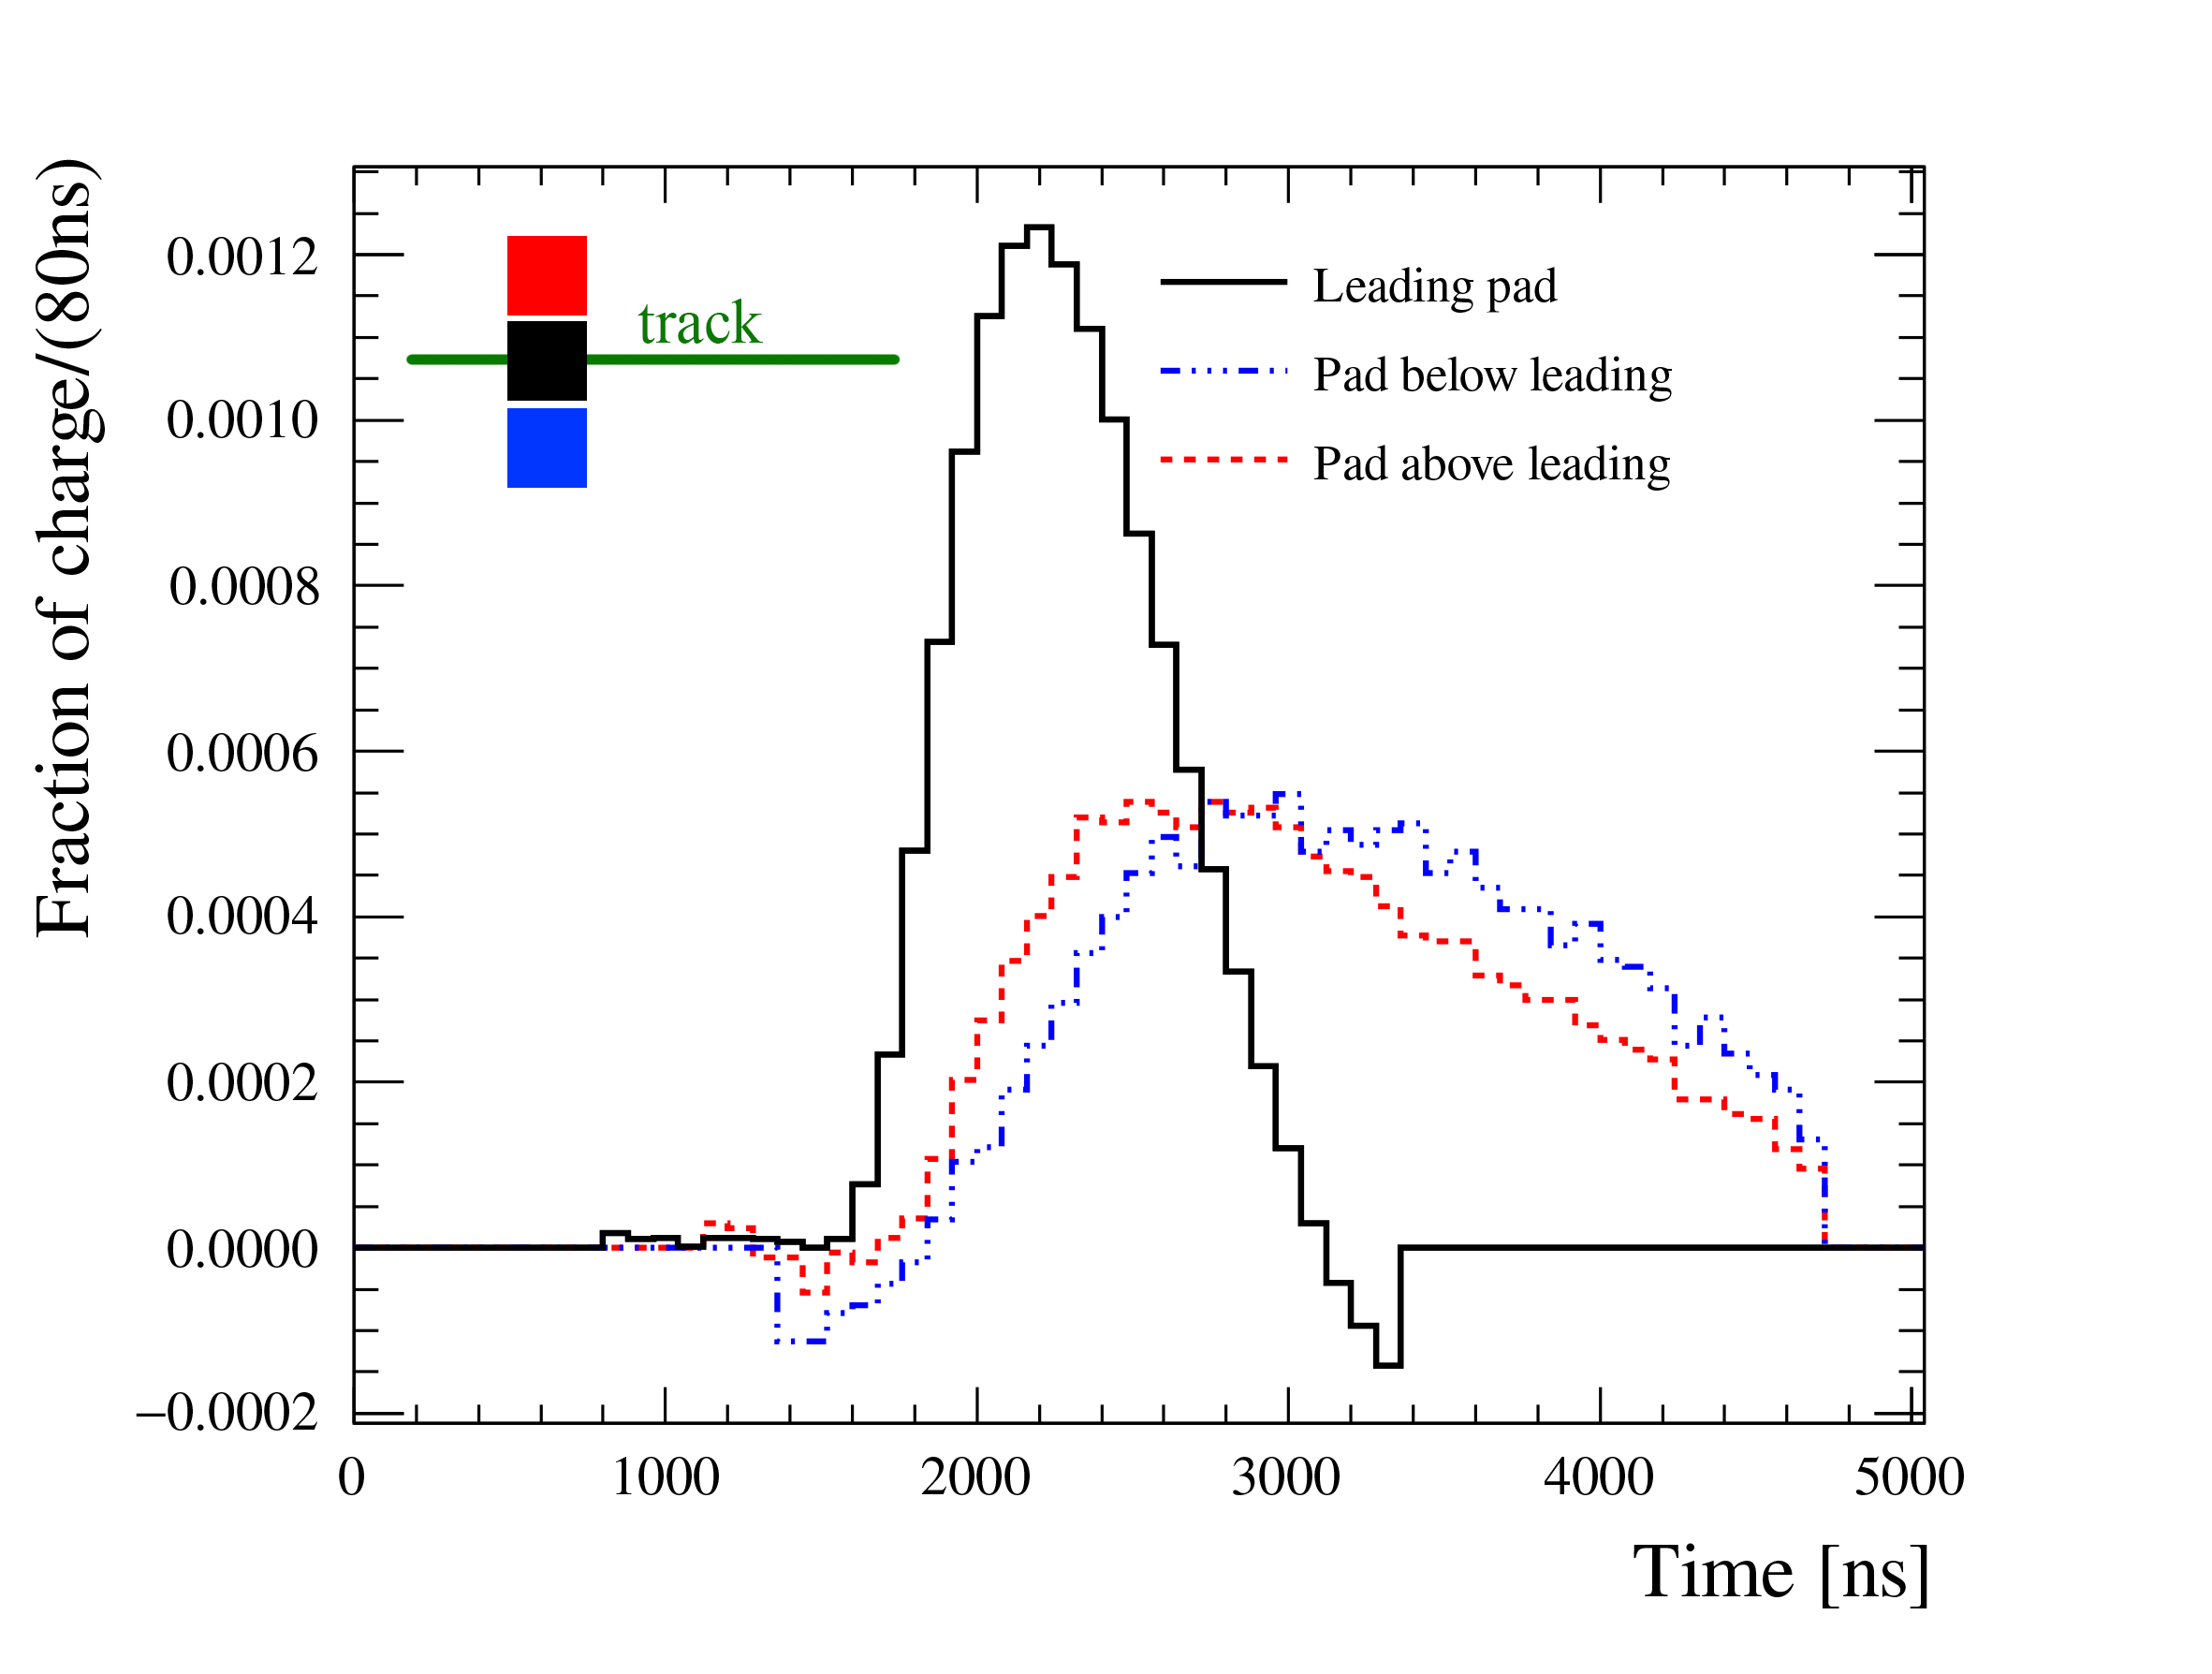
\includegraphics[width=0.6\linewidth]{cern_wf}
   \caption{The waveform recorded in the three neighbor pads. The tracks went over the pad shown in black and the resistive foil spread the charge to the pad below and above (blue and red) with some delay in time.}
   \label{fig:tpc:cern_wf}
 \end{figure}

\subsubsection{Track reconstruction}
A simple algorithm was developed to reconstruct the cosmic and beam tracks. With the beamline intensities, several particles can cross the TPC within one event. I expect a through-going track to be a continuous chain of hits between the Micromegas edges. The track reconstruction starts with a selection of groups of pads at the beginning and at the end of the Micromegas. Relatively high threshold of 50 charge unit is set to suppress all the noisy pads. The pads that are illuminated with charge spreading are suppressed as well. At this step I'm interested only in the pads that are crossed by the track. Then the algorithm looks for all the possible connections between these clusters. Again, a high threshold is applied to deal with primary pads only and do not take into account charge sharing. The sharing is essential for the precision track positioning, but not for the pattern recognition. Delayed pads can make a confusion and result in merging of two different tracks. If there is a chain of hits connecting these clusters in three dimensions such a chain will be recognized as a track. After that, the time window in space and time is defined ``around'' the track. I'm looking for hits on both sides and with possible time delay up to 2.5 $\mu$s. The pads of the side of the track that where triggered before the central one are not considered as a charge spreading should be delayed.

At our energies, most of the tracks are straight lines. There are very few events with complicated topologies like decays or scatterings and such events were omitted.  I put a cut on the maximum number of clusters at the beginning and at the end of the track. If it's more than four, the event seems to be too complicated to perform an accurate reconstruction and is omitted. If the tracks width is more then six pads, the track is omitted as well. I observed that normal tracks do not spread more then five pads and when the large spreading happens it clearly indicates that there was some kind of reaction, scattering or a delta---ray emission.

An example of a raw event with two tracks is presented in figure \autoref{fig:tpc:cern_ph} (a). With our algorithm, we extracted the bottom track and omitted the upper one as we suspect some interaction that causes the large charge deposition with a spreading up to 7 pads in width.

\begin{figure}[!ht]
  \centering
  \begin{minipage}{0.49\linewidth}
    \centering
    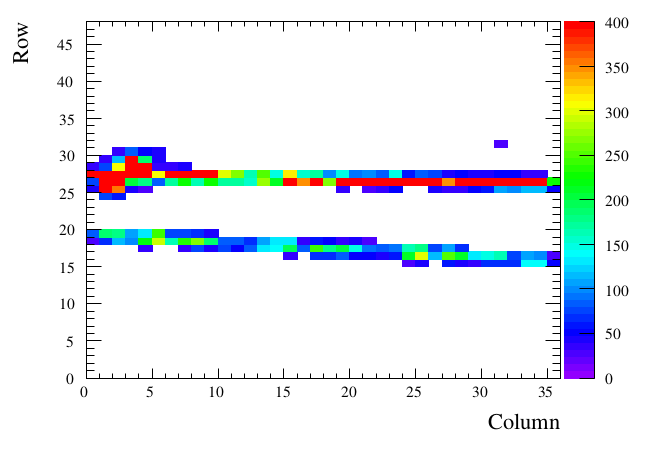
\includegraphics[width=0.8\linewidth]{cern_tpc_raw} \\ (a)
  \end{minipage}
  \begin{minipage}{0.49\linewidth}
    \centering
    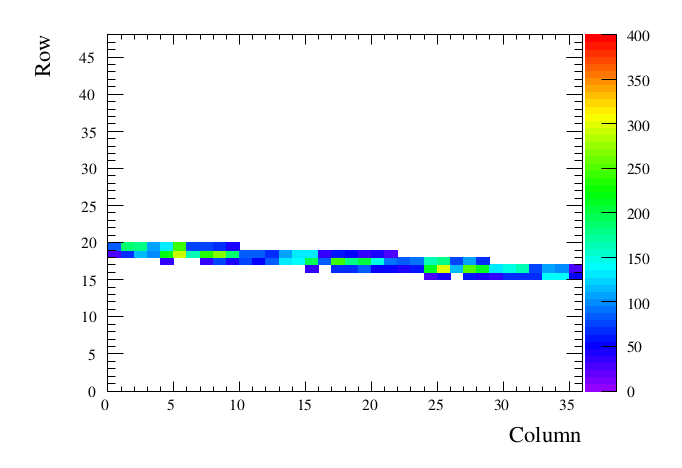
\includegraphics[width=0.8\linewidth]{cern_tpc_sel} \\ (b)
  \end{minipage}
  \caption{The example of the raw event (a) and the extracted track of interest (b) in the TPC prototype.}
  \label{fig:tpc:cern_ph}
\end{figure}

\subsubsection{Gas quality}
The gas quality is an important characteristic of the TPC. We performed its checks with the drift velocity, attenuation length and gain measurements.

The drift velocity is a convenient metric of the gas mixture quality. The stability of the drift velocity is an essential characteristic of the mixture for the precise analyses. For the drift velocity measurements, we used cosmic tracks that were intersecting a cathode or Micromegas. It was possible since the scintillator bars used for the cosmic trigger system were wider than the detector drift region. Such tracks can be recognized with a start or endpoint in the middle of the detector plane. The timestamps of the anode/cathode crossings are presented in \autoref{fig:tpc:cern_drift} (a). The different amount of tracks at each end was caused by the significantly lower acceptance of the cosmic trigger for tracks close to the anode. The time difference between two peaks will give us an electron drift time for the given drift distance of the 150 cm. The evolution of the drift velocity is shown in \autoref{fig:tpc:cern_drift} (b).

\begin{figure}[!ht]
  \centering
  \begin{minipage}{0.49\linewidth}
    \centering
    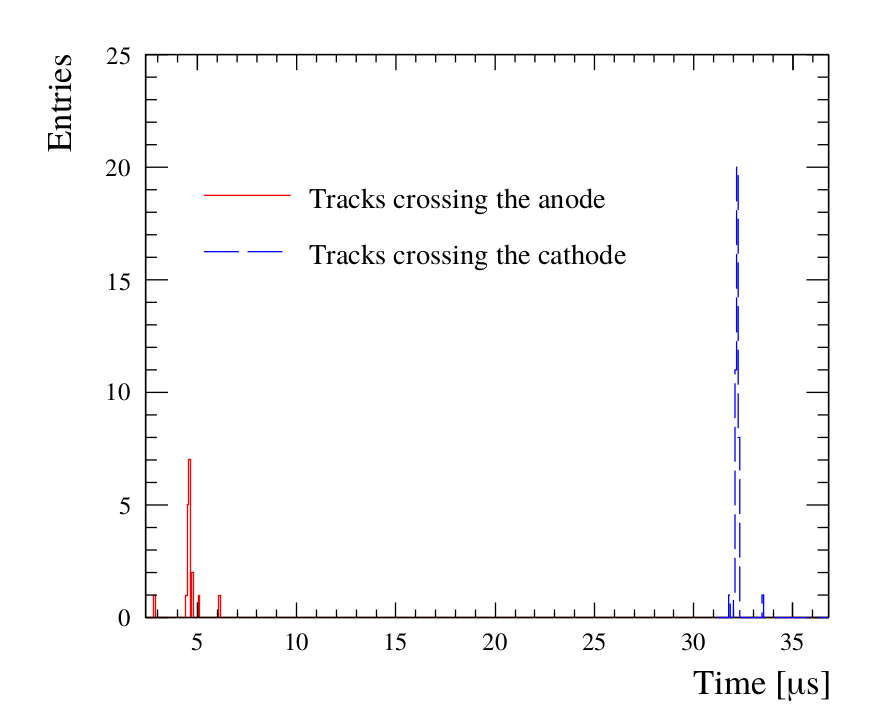
\includegraphics[width=0.8\linewidth]{cern_time_cross} \\ (a)
  \end{minipage}
  \begin{minipage}{0.49\linewidth}
    \centering
    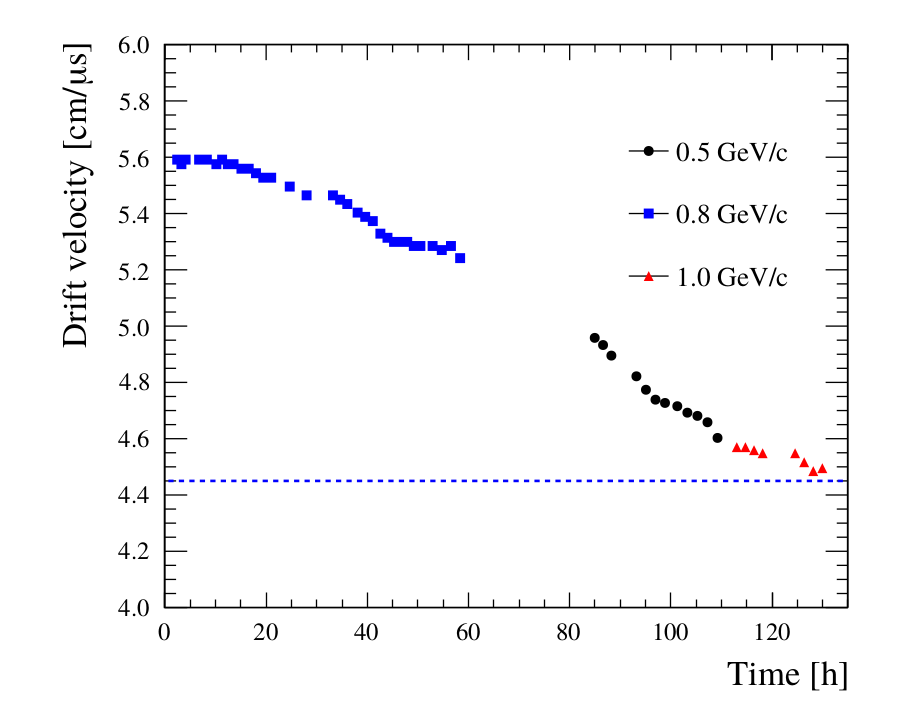
\includegraphics[width=0.8\linewidth]{cern_drift} \\ (b)
  \end{minipage}
  \caption{The drift velocity measurements in the TPC prototype in CERN beamtest. (a) The timestamps of the cathode/Micromegas intersection and (b) the estimated values  of the drift velocity.}
  \label{fig:tpc:cern_drift}
\end{figure}

The attenuation length is another characteristic of gas quality. It shows how many electrons were absorbed during the drift. Lower attenuation length will result in the lower measured charge and will affect more the tracks that are away from Micromegas. We used cosmic tracks for this measurement as they crossed the TPC at all the range of drift distances. The mean collected charge versus the drift distance was fit with the exponential law to extract the attenuation length. The illustration of the attenuation effect and the evolution of the attenuation length during the data taking are shown in \autoref{fig:tpc:cern_att}. A slight degradation was observed but it was always at least twice the TPC length and would not cause a degradation of the data quality.

\begin{figure}[!ht]
  \centering
  \begin{minipage}{0.49\linewidth}
    \centering
    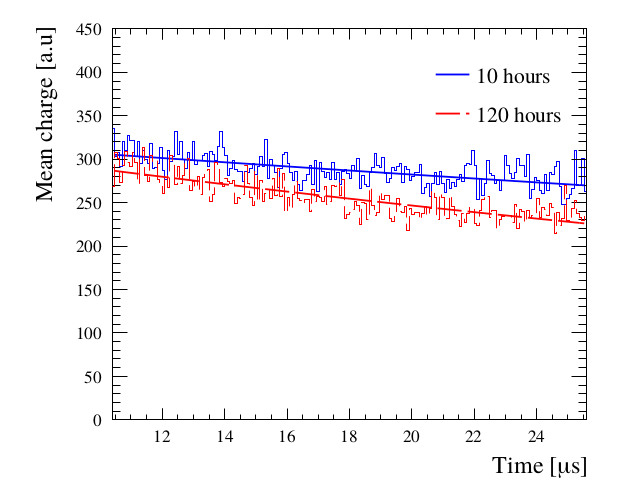
\includegraphics[width=0.8\linewidth]{cern_att} \\ (a)
  \end{minipage}
  \begin{minipage}{0.49\linewidth}
    \centering
    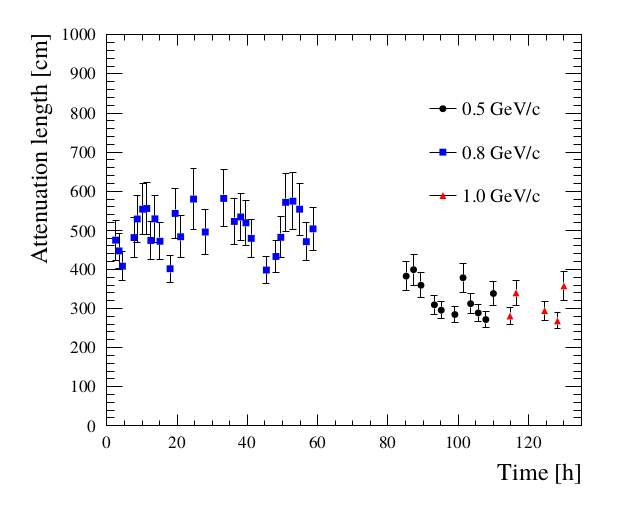
\includegraphics[width=0.8\linewidth]{cern_att_2} \\ (b)
  \end{minipage}
  \caption{The attenuation effect in the TPC prototype at the beamtest at CERN (a) and the attenuation length during the data taking (b). The measurements were done with the cosmic tracks, the momentum of the beam is illustrating what data sample were taken with the beam at that time.}
  \label{fig:tpc:cern_att}
\end{figure}

The gain evolution during the data taking was measured using the ${}^{55}\text{Fe}$ source. The radioactive source was mounted at the center of the cathode. For each event triggered by either cosmic or a beam trigger the time window for data recording is more than the drift time for the whole TPC length. During that time we expect to detect about two ${}^{55}\text{Fe}$ decays with 5.9 keV X-ray emission. Therefore no special trigger was needed and the clusters from the source decays can be found in the beam or cosmic data. The total charge collected from the cluster was used for the gain estimations. The gain itself is computed as a ratio of the measured electrons to initial electrons from X--ray interaction. From the 5.9 keV photon interaction with Argon, 230 initial electrons are expected. This value was measured in the various gaseous detectors' tests and used as an input in our analyses. The whole dynamic range of each pad is 4096 channels that correspond to the total charge of 120 fC. The measured spectrum for the radioactive source is shown in \autoref{fig:tpc:cern_gain} (a). A resolution was good enough to see also a 2.9 keV escape line in Argon. The gain was expected to depend on the Micromegas voltage with an exponential law. The expected dependence was observed during the MM high voltage scan (\autoref{fig:tpc:cern_gain} (b)). The gain evolution with a constant MM voltage during the data taking is shown in \autoref{fig:tpc:cern_gain} (c). The gain value depends on the gas quality (e.g. water contamination), atmospheric pressure and temperature. All these parameters were not precisely controlled during the data taking thus fluctuations were possible.

\begin{figure}[!ht]
  \centering
  \begin{minipage}{0.33\linewidth}
    \centering
    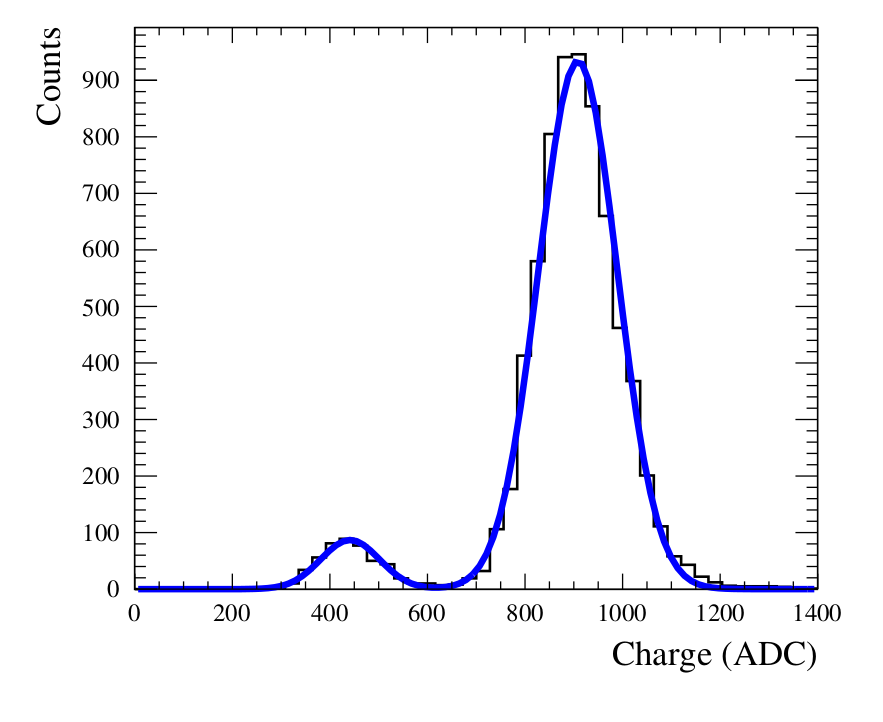
\includegraphics[width=\linewidth]{cern_iron} \\ (a)
  \end{minipage}
  \begin{minipage}{0.33\linewidth}
    \centering
    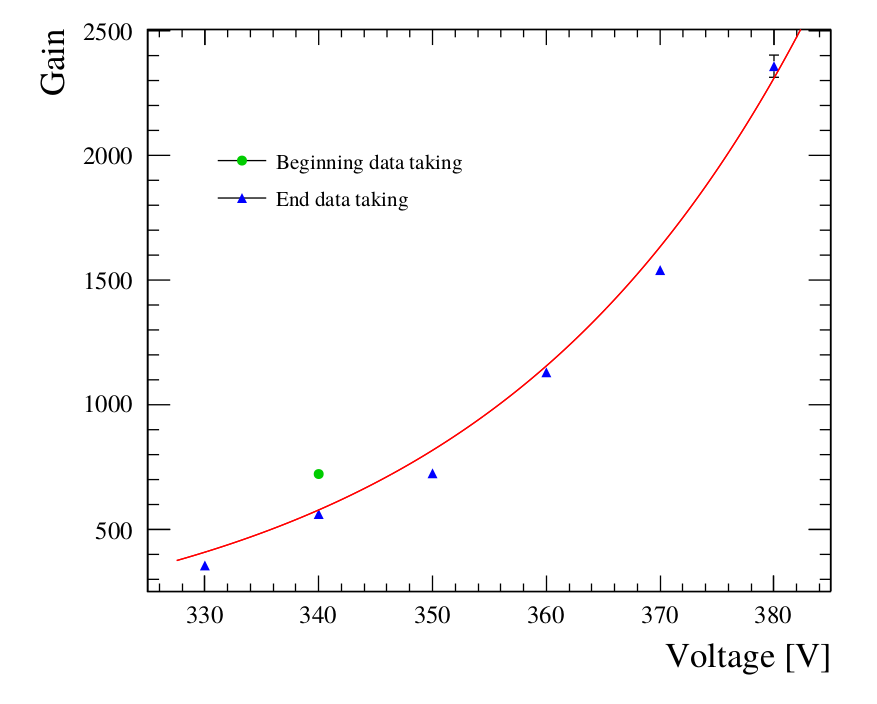
\includegraphics[width=\linewidth]{cern_gain_v} \\ (b)
  \end{minipage}
  \begin{minipage}{0.33\linewidth}
    \centering
    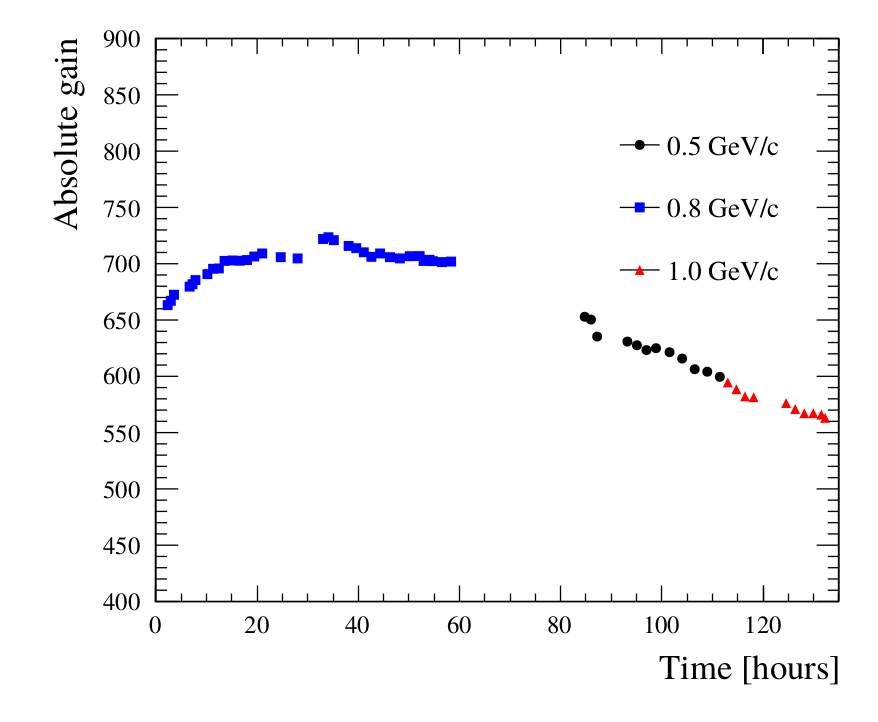
\includegraphics[width=\linewidth]{cern_gain} \\ (c)
  \end{minipage}
  \caption{The spectrum of the ${}^{55}\text{Fe}$ source with measured 5.9 keV X--ray and 2.9 keV escape line in Argon (a). The evaluation of the gain versus the Micromegas voltage (b) and versus the data taking period (c)}
  \label{fig:tpc:cern_gain}
\end{figure}

For all the measurements of the gas parameters, we observed a slight improvements of the gas quality at the very beginning with further degradation with time. We assume that the degradation was due to increasing $\text{H}_2\text{O}$ contamination in the mixture. Water is known to slow down the electron drift, increase the attenuation and reduce the gain. The HARP field cage was stored in the air for a long time and was not dried before the operation. During the test the TPC was operated in overpressure, thus we consider that the gas quality degradation was caused by the water releasing from the field cage. The evolution of the gas parameters during the beamtest was correlated with the change of the gas flow in the detector. At the beginning of the data taking the flow was set to 60 L/h and was further decreased to 25 L/h as the mixture was believed to be stable enough. During the data analyses, it was found that the gas flow reduction caused the degradation of the mixture parameters. However, this degradation is not critical for the measurements. For the data analyses, the corrections were applied to compensate for the gain and attenuation length drop.

\subsubsection{Ionization energy loss (dE/dx) resolution}
\label{sec:tpc:tpc_dedx}
The dE/dx resolution is critical for the T2K measurements. As mentioned in \autoref{sec:t2k:tpc} of \autoref{ch:T2K:general}, during the ionization process charged particles lose the energy with high fluctuations. The average value of several independent measurements is used for the particle type estimations. The resistive foil usage implements a correlation of the measured charge values in the neighbor pads. It can spoil the dE/dx resolution as each measurement is not independent anymore. I estimated the dE/dx resolution for the beam tracks with the CERN TPC prototype.

The dE/dx resolution was measured with the horizontal beam tracks. The track is considered as a group of ``clusters''. The ``cluster'' is defined as a group of pads perpendicular to the track direction. E.g. for the horizontal track the hits in a particular column of the Micromegas will form a ``cluster''. The charge collected in the cluster is summed up and considered as an energy loss per fixed length (0.9 mm --- pad size). The distribution of the charge per cluster has a long tail towards the high energy. This is in agreement with the expected ionization energy spectrum as it is described with Landau distribution. To omit the clusters with large charge deposition the ``truncation'' method is used. All the clusters in the track are sorted by increasing charges. Some clusters from the beginning of the list (e.g. 70\%) are used to estimate the average energy loss per cluster. The truncation fraction is varied to obtain the best dE/dx resolution. The 62.5\% truncation was found to provide the best performance (\autoref{fig:tpc:cern_energy_1} (a)). The average energy loss per unit length before and after the truncation is shown in \autoref{fig:tpc:cern_energy_1} (b). As one can see the distribution becomes Gaussian. Therefore the mean and the standard deviation can be estimated and the resolution can be computed.

\begin{figure}[!ht]
  \centering
  \begin{minipage}{0.49\linewidth}
    \centering
    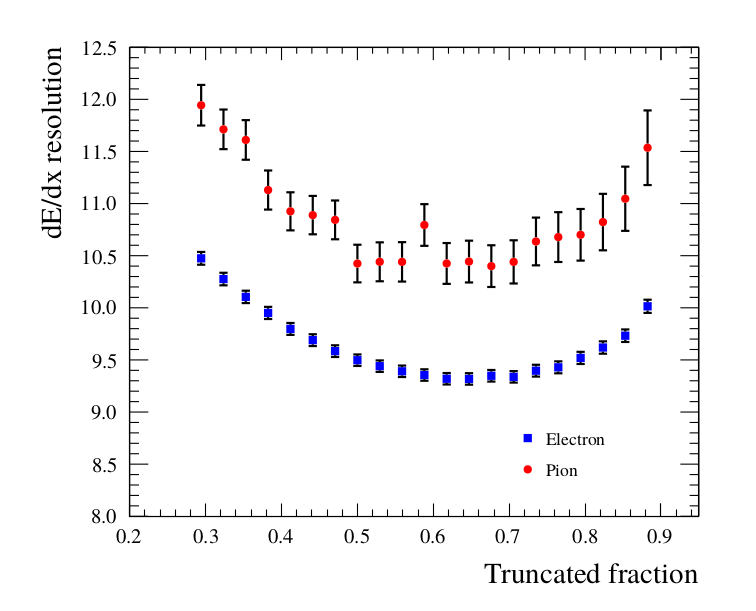
\includegraphics[width=\linewidth]{cern_truncation} \\ (a)
  \end{minipage}
  \begin{minipage}{0.49\linewidth}
    \centering
    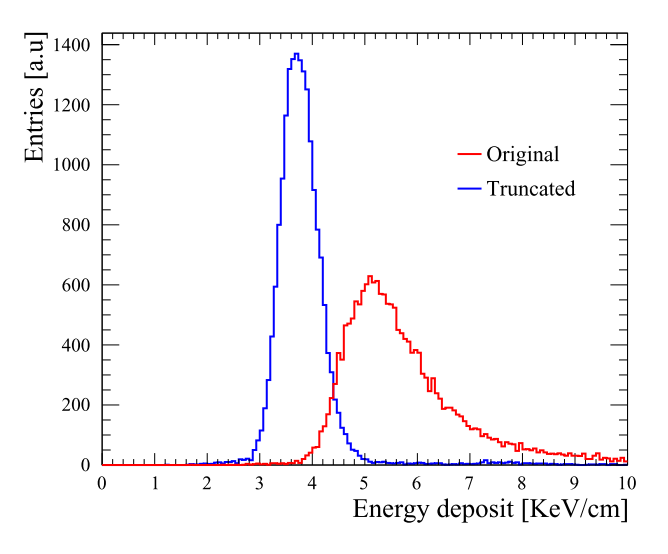
\includegraphics[width=\linewidth]{cern_trunc_ex} \\ (b)
  \end{minipage}
  \caption{Resolution on the energy deposit per unit of track length for different truncation values (a). Comparison on the energy deposited per unit length on the same beam sample of positrons at 0.8 GeV/c with and without applying the truncation mean method (b).}
  \label{fig:tpc:cern_energy_1}
\end{figure}

The dE/dx distributions for 0.8 GeV/c electrons, pions and protons samples are shown in \autoref{fig:tpc:cern_energy_2} (a). The particle type per each sample is defined based on the trigger combination that was used. However, the contamination of other particle types is possible. The pion sample has two peaks, and the second peak matches perfectly with the peak in the electron sample. As the electrons are dominating in the beam, we suspected that a small impurity in the pion trigger can cause the acceptance of the electrons. The resolution for each particle sample and drift distance is shown in \autoref{fig:tpc:cern_energy_2} (b). For the pion sample, only the first peak that indeed corresponds to the pion is used. The results are summarized in \autoref{tbl:tpc:cern_dedx}. The worse resolution in the pion sample is understood as they are less ionizing comparing to protons or electrons. Less deposited charge is more affected by the fluctuations. Scaling of the obtained results to the twice longer ND280 TPC will give us a performance similar to one at the existing detectors. That is a very important conclusion as we were afraid of the dE/dx resolution degradation with the resistive anode technology.

\begin{figure}[!ht]
  \centering
  \begin{minipage}{0.49\linewidth}
    \centering
    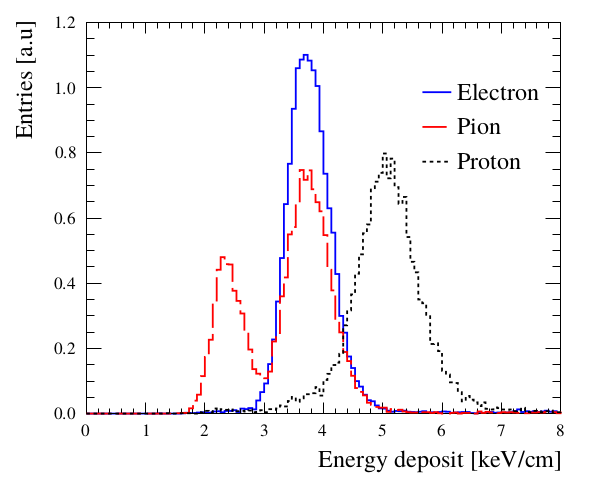
\includegraphics[width=\linewidth]{cern_energy} \\ (a)
  \end{minipage}
  \begin{minipage}{0.49\linewidth}
    \centering
    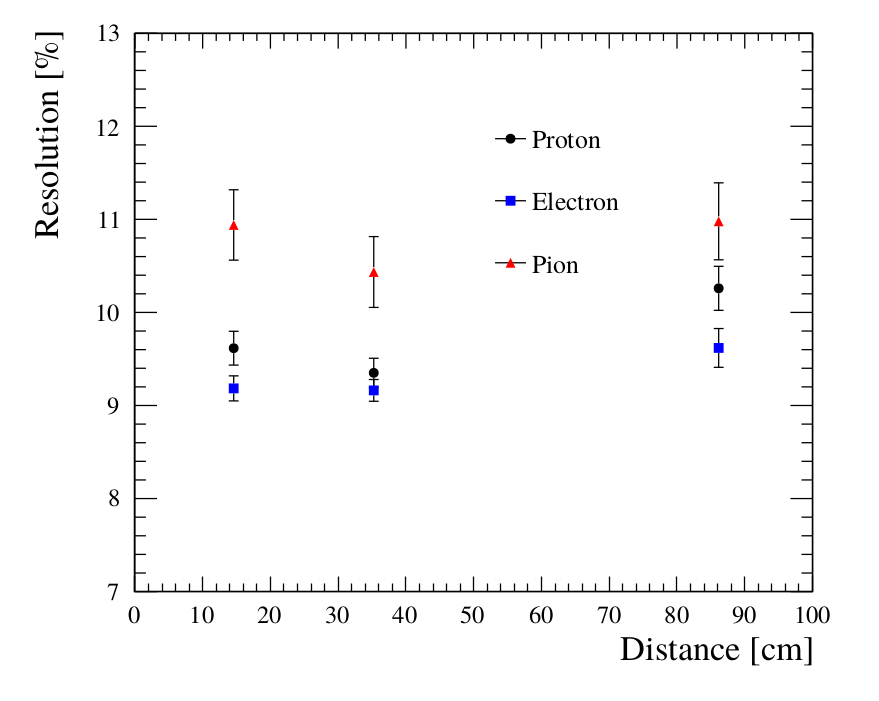
\includegraphics[width=\linewidth]{cern_energy_resol} \\ (b)
  \end{minipage}
  \caption{The dE/dx resolution for different particles samples and drift distances (b) obtained from the dE/dx distributions for each sample (a) in the TPC prototype test at CERN.}
  \label{fig:tpc:cern_energy_2}
\end{figure}

\begin{table}[!ht]
  \centering
  \begin{tabular}{|l|c|}
  \hline
  \hline
  Sample    & Resolution, \% \\
  \hline
  Electron  & $9.2\pm0.1$ \\
  Pion      & $10.9\pm0.4$ \\
  Proton    & $9.6\pm0.2$ \\
  \hline
  \end{tabular}
  \caption{The dE/dx resolution for different particles samples at 10 cm drift distance.}
  \label{tbl:tpc:cern_dedx}
\end{table}

\subsubsection{Spatial resolution}
The spatial resolution analyses is extremely important as we expect a noticeable improvement comparing to the existing TPCs. With the resistive Micromegas the charge is shared between few pads that allows more accurate position reconstruction (\autoref{fig:up:res}). The easiest method to extract the position based on the signal in a few pads is a weighted mean. The description of the method is provided in \autoref{eq:tpc:coc}. The group of pads perpendicular to the track direction is referred to as a ``cluster''. In our beamtest particles provide horizontal track, therefore each column is a ``cluster''. In the cluster, all the pads are weighted with the measured charge and the weighted mean will give a track position in the particular cluster.
\begin{equation}
\label{eq:tpc:coc}
x_{track} = \frac{\sum (x_{pad} \cdot Q_{pad})}{\sum Q_{pad}}
\end{equation}

The track position in all the clusters can be further fit with a straight line or with an arc in the presence of the magnetic field. It was proved that such a method demonstrates the resolution improvement comparing to the existing TPCs~\cite{Dixit2004}. But there is room for further improvement. The charge spreading is described with the exponential law. With the weighted mean, we sample the exponential distribution in large bins. The pad size is a few times bigger than the standard deviation of the charge spreading. With the weighted mean the whole charge collected in the pad is assigned to the pad center while with the exponential distribution of the charge it behaves differently. The improved method of the spatial resolution estimation is based on a so--called ``pad response function'' (PRF) that is used to describe the spreading of the charge. It was implemented in the ILC prototype analyses and was proved to improve the result over the weighted mean~\cite{Attie2011}.

By definition, the PRF function describes the fraction of the cluster charge deposited in the particular pad versus the distance between the track and pad center.

\begin{equation}
Q_{pad}/Q_{cluster} = PRF\left(x_{track} - x_{pad}\right)
\label{eq:prf_def}
\end{equation}

Assuming the PRF is known, we can compare the measured $Q_{pad}/Q_{cluster}$ with the expectations for the given track position. And the best track position in the cluster can be chosen based on the $\chi^2$ fit.

\begin{equation}
\label{eq:tpc:chi2}
\chi^2=\sum_{pads}\frac{Q_{pad}/Q_{cluster} - PRF\left(x_{track} - x_{pad}\right)}{\sigma}
\end{equation}
where $\sigma$ is an uncertainty of the $Q_{pad}/Q_{cluster}$. I assumed the charge deposition follows the Poisson distribution and therefore the uncertainties can be estimated with $\sigma=\sqrt{Q_{pad}}/Q_{cluster}$. To extract the track position the PRF shape should be known , but to estimate the PRF we need the information about the track position. To deal with it I used the weighted mean method as a prior guess about the track position. Based on the known information the PRF scattered plot is filled (\autoref{fig:tpc:prf} (a)). Then the obtained 2D histogram is profiled. In the 1D slice along the Y axis (\autoref{fig:tpc:prf} (b)) the maximum is interpreted as a PRF value and the width at the half maximum as an uncertainty. As a result, I obtained 1D graph that can be fit with the analytical function (\autoref{fig:tpc:prf} (c)). For the analytical function, the 4-th order polynomial was chosen.

\begin{equation}
PRF(x, \Gamma, \Delta, a, b)=\frac{1+a_2x^2+a_4x^4}{1+b_2x^2+b_4x^4}
\label{eq:GL}
\end{equation}

The coefficients $a_2$ and $a_4$, and $b_2$ and $b_4$ can be expressed in terms of the full width half maximum $\Gamma$, the base width $\Delta$ of the PRF, and two scale parameters $a$ and $b$.

\begin{figure}[!ht]
  \centering
  \begin{minipage}{0.33\linewidth}
    \centering
    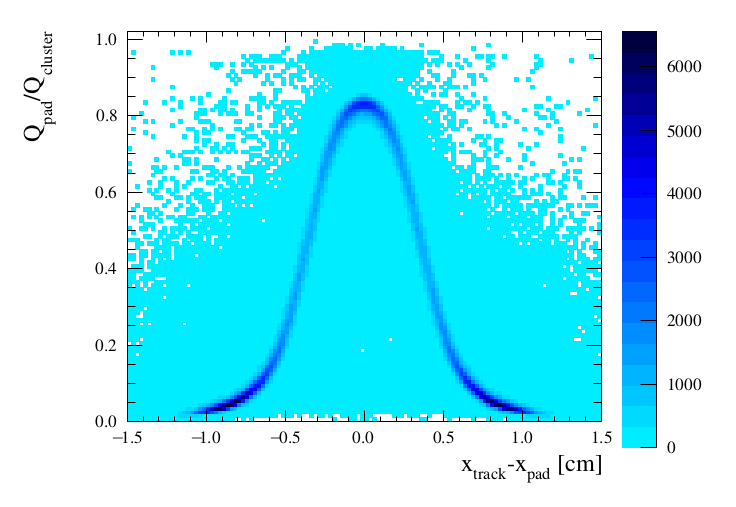
\includegraphics[width=\linewidth]{prf_sc} \\ (a)
  \end{minipage}
  \begin{minipage}{0.33\linewidth}
    \centering
    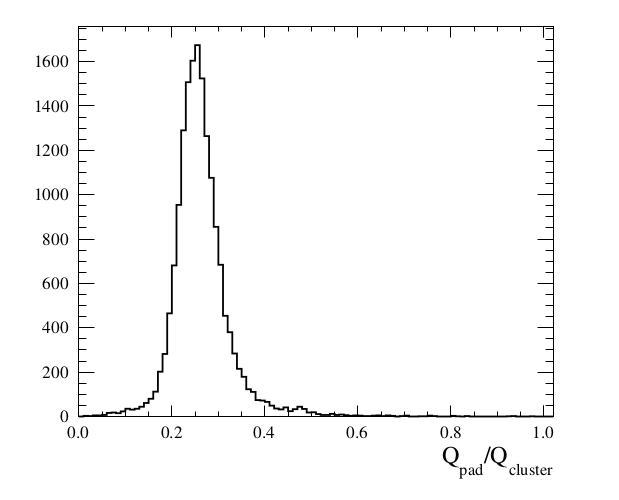
\includegraphics[width=\linewidth]{prf_pr} \\ (b)
  \end{minipage}
  \begin{minipage}{0.33\linewidth}
    \centering
    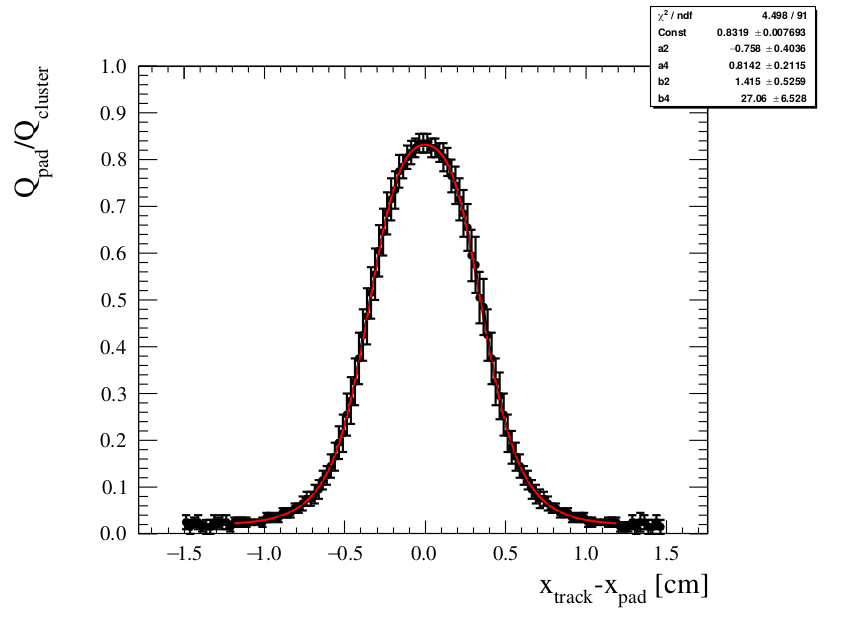
\includegraphics[width=\linewidth]{prf_func} \\ (c)
  \end{minipage}
  \caption{The PRF estimations steps: 2D scatter plot filled with each track cluster (a), the 1D slice for particular value of $x=-0.5$ (b) and a 1D graph that can be fit with the analytical function.}
  \label{fig:tpc:prf}
\end{figure}

The spatial resolution analyses flow looks as following:
\begin{enumerate}
  \item Start with the weighted mean as a prior:
  \begin{enumerate}
    \item track position in each cluster is evaluated with weighted mean
    \item positions in the cluster are fit together to form a track
    \item the PRF scatter plot is filled for each pad with $X_{track} - X_{pad}$ and $Q_{pad}/Q_{cluster}$
  \end{enumerate}
  \item PRF scatter plot is profiled to the graph and fit with the analytical function
  \item PRF method:
  \begin{enumerate}
    \item track position in each cluster is evaluated with $\chi^2$ fit (\autoref{eq:tpc:chi2})
    \item positions in the cluster are fit together to form a track
    \item the PRF scatter plot is filled for each pad with $X_{track} - X_{pad}$ and $Q_{pad}/Q_{cluster}$
  \end{enumerate}
\end{enumerate}

To estimate the spatial resolution the residuals are defined as a difference between the global track fit and position reconstructed in the particular cluster. The residuals are fit with the Gaussian function. The spatial resolution and bias are defined as sigma and mean of the fit respectively. Steps 2 and 3 are repeated while the spatial resolution is improving. The spatial resolution and the bias obtained with weighted mean and PRF are shown in \autoref{fig:tpc:cern_sr}. The PRF method provides a much more accurate result over the weighted mean. Also, it is more uniform over the detector. The resolution across all particle types and drift distances is presented in \autoref{fig:tpc:sr_tot}. As was expected protons have a better resolution as they deposit more charge and the position can be estimated more precisely. Also, I observed the expected degradation of the spatial resolution with the increase of the drift distance. Because of the transversal diffusion the electron cloud becomes wider during the drift and the position reconstruction accuracy decreases. Finally, I observed the accuracy at the level of 250 $\mu\text{m}$ for the 10 cm drift distance. In the existing T2K TPC the resolution is at the level of 750 $\mu\text{m}$ at the same distance. The resistive foil was confirmed to improve the precision without changing the pad size.

The dependence of the spatial resolution on the drift distance is an important characteristic of the resistive TPC. Without a resistive layer, the resolution becomes worse with decreasing the drift distance. That happens because the transverse diffusion is not sufficient to spread the charge to more then one pad. All the charge is collected by one pad, thus the uncertainty of the measurement is limited by its size. The analytical study of the spatial resolution dependence on the drift distance is provided in~\cite{Arogancia2009}. The advantage of the resistive Micromegas is a charge spreading in the resistive foil, therefore more than one pad receive the signal even for a track close to the readout plane. The spatial resolution for such a detector is expected to follow the square root dependence with respect to the drift distance ($z$). The dependence of the resolution is given by \autoref{eq:up:tpc:sr}~\cite{Dixit2007}.

\begin{equation}
\label{eq:up:tpc:sr}
  \sigma\left(z\right)=\sqrt{\sigma_0^2+\frac{D^2_{Tr}z}{N_{eff}}}
\end{equation}
where $\sigma_0$ is the resolution at zero drift distance, $D_{Tr}$ is the transverse diffusion constant, and $N_{eff}$ is the effective number of electrons over the length of pad. $N_{eff}$ is computed based on the number of initial ionization electrons $N$ with $N_{eff}=1/\langle\sqrt{1/N}\rangle^2$.

Thus, improving the spatial resolution with the reduction of the drift distance is a clear effect of the resistive foil.

\begin{figure}[!ht]
  \centering
  \begin{minipage}{0.49\linewidth}
    \centering
    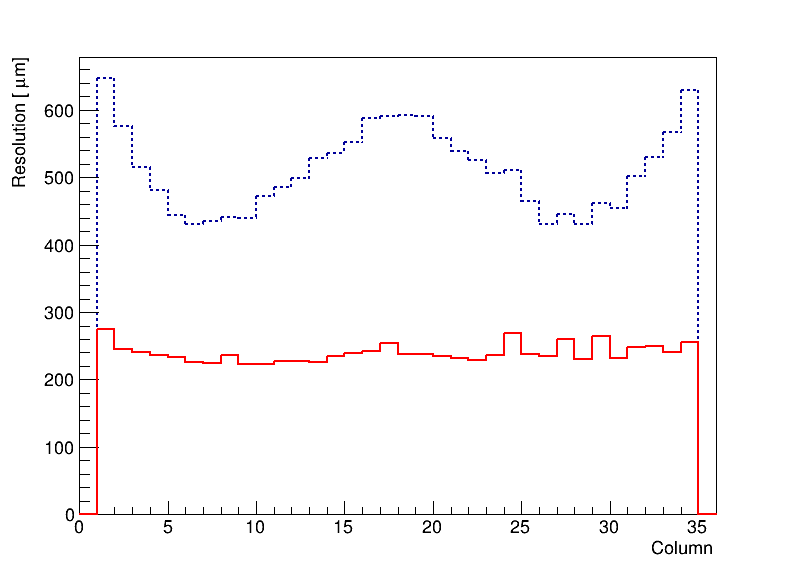
\includegraphics[width=0.8\linewidth]{cern_impr} \\ (a)
  \end{minipage}
  \begin{minipage}{0.49\linewidth}
    \centering
    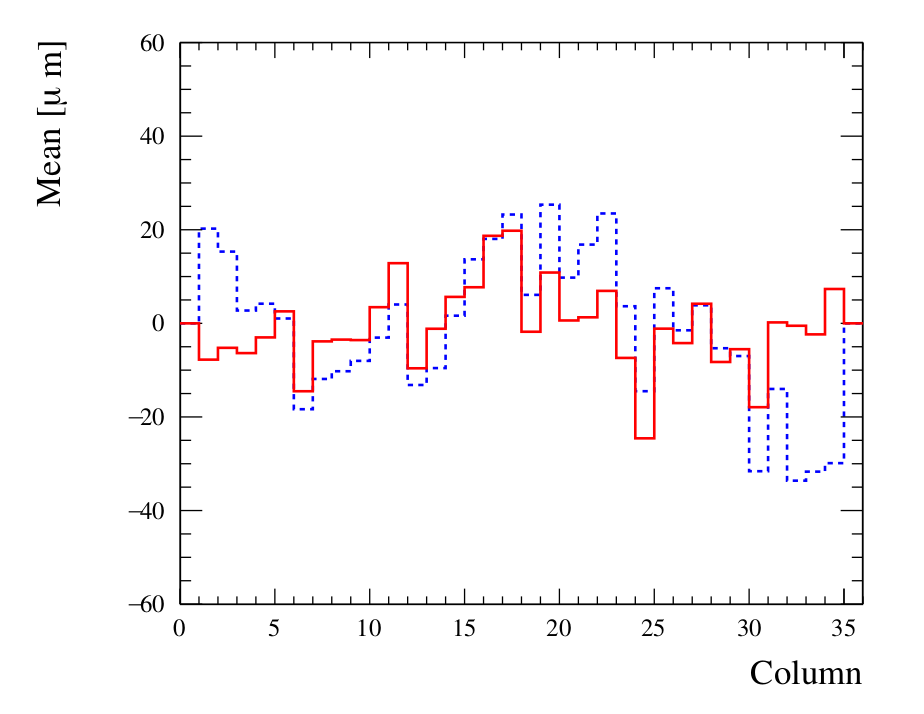
\includegraphics[width=0.8\linewidth]{cern_bias} \\ (b)
  \end{minipage}
  \caption{The spatial resolution (a) and a bias (b) obtained in the TPC prototype test at CERN with 10 cm drift distance with electron sample. The results of the weighted mean method are shown in dashed blue and the results from PRF method is solid red.}
  \label{fig:tpc:cern_sr}
\end{figure}

\begin{figure}[!ht]
  \centering
  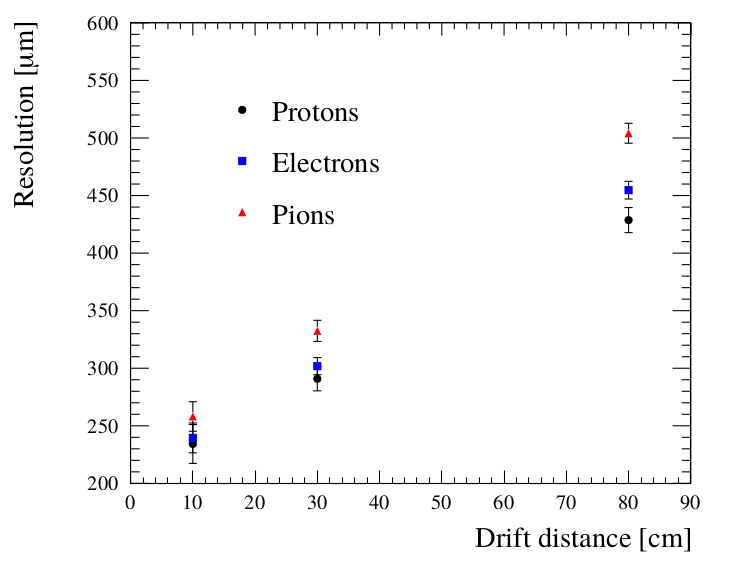
\includegraphics[width=0.5\linewidth]{cern_res}
  \caption{The spatial resolution for all the particles types and drift distances in the CERN beam test.}
  \label{fig:tpc:sr_tot}
\end{figure}

The beamtest at CERN shows good performance of the resistive TPC prototype. Different samples with different particles types and at various drift distances were tested. The dE/dx resolution was estimated at the same level as in existing TPCs but the spatial resolution was proved to be significantly improved. The paper describing the analyses and the results I obtained was published~\cite{Attie2019b}.

\subsection{DESY beamtest}
The CERN beamtest confirms the good performance of the new detector. The tested detector was based on the same circuit board (PCB) as we are using in the ND280 TPCs at the moment. The planned HA--TPCs will have different dimensions and pad sizes. The new micromegas was produced for the next beamtest. The same dimensions as in HA--TPC were used. The module size is $\text{34}\times\text{42}\text{ cm}^2$ and is paved with $\text{32}\times\text{36}$ pads $\text{1.1}\times\text{1.0}\text{ cm}^2$ each. The thin 75 $\mu\text{m}$ insulator layer is covered with 50 $\mu\text{m}$ Kapton with the DLC on top of it. Compared to the first prototype (200 + 50 $\mu\text{m}$) the capacitance was increased. The resistivity was decreased from 2.5 $M\Omega/\square$ down to 0.4 $M\Omega/\square$. The side pads were partly covered for mesh fixation as before and these pads were excluded from the analyses.

The DESY beamtest facility provides a beam of electrons. The momentum can be adjusted from 1 to 5 GeV/c. The scheme of the beamtest facility is provided in \autoref{fig:tpc:desy_beam}. A magnetic field was used in this test. Most of the samples were taken with 0.2 T field strength, while some data were collected in the absence of the field.

\begin{figure}[!ht]
  \centering
  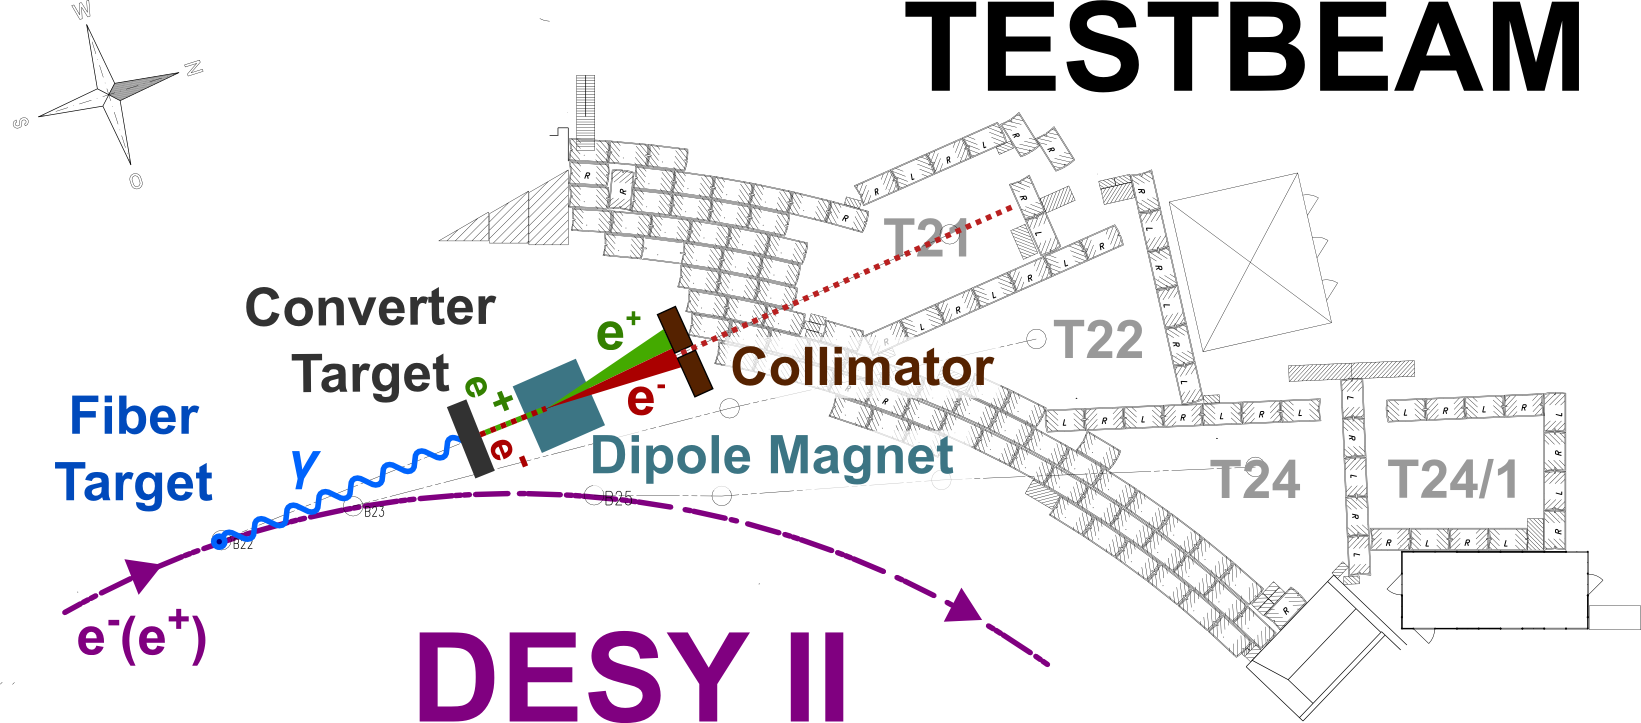
\includegraphics[width=0.7\linewidth]{desy_beam}
  \caption{The scheme of the DESY beamtest facility}
  \label{fig:tpc:desy_beam}
\end{figure}

\subsubsection{Track reconstruction}
In addition to the track reconstruction method described in the CERN test section, we also tried the DBSCAN (Density-Based Algorithm for Discovering Clusters) algorithm~\cite{Ester1996}. As it is aimed at matching the hits into clusters based on the hit ``weight'', it looks like a good framework for our case. In the CERN beamtest it was found excessive and was not used for the final result, but in the DESY analyses it demonstrated better performance and was chosen as the main algorithm. The examples of the reconstructed tracks are shown in \autoref{fig:tpc:desy_tracks}.

\begin{figure}[!ht]
  \centering
  \begin{minipage}{0.49\linewidth}
    \centering
    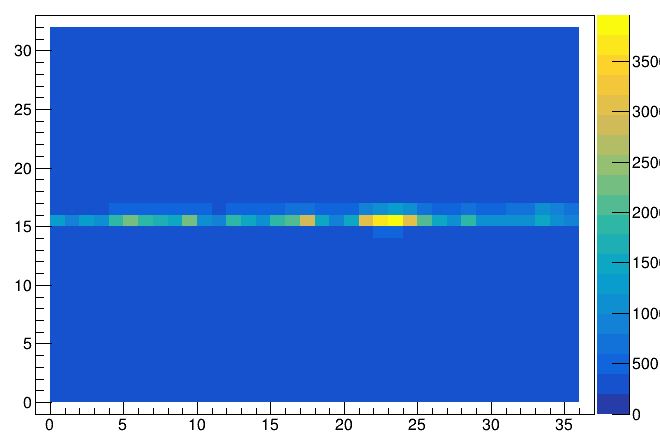
\includegraphics[width=\linewidth]{DESY_ed_1}
  \end{minipage}
  \begin{minipage}{0.49\linewidth}
    \centering
    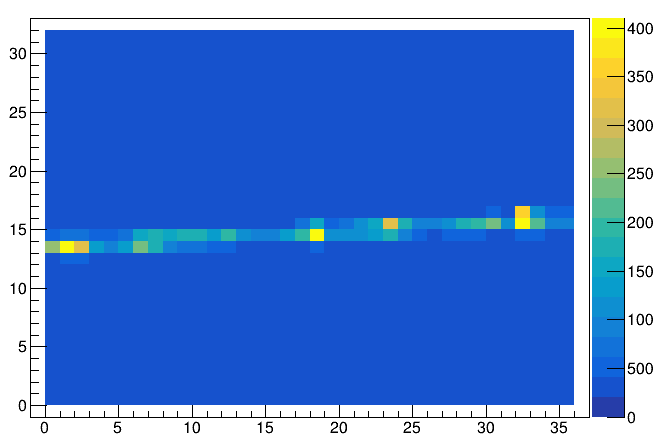
\includegraphics[width=\linewidth]{DESY_ed_2}
  \end{minipage}
  \caption{Two examples of the reconstructed tracks from the DESY beamtest.}
  \label{fig:tpc:desy_tracks}
\end{figure}

\subsubsection{Ionization energy loss resolution}
The dE/dx resolution was tested with the same method as was used for CERN and Saclay analyses. The truncated mean of the charge collected from the track distribution was fit to estimate the resolution. In the CERN beam test analyses I observed mostly two pads per cluster. We suspect that not sufficient charge spreading may limit the spatial resolution. In the DESY test the nominal MM voltage was increased to 360 V. The effect of the high voltage on the multiplicity can be seen in \autoref{fig:tpc:desy_mult}. Thus with the nominal voltage I observed 3 pads per cluster in most of the cases. With this I expected to improve the spatial resolution.

\begin{figure}[!ht]
  \centering
  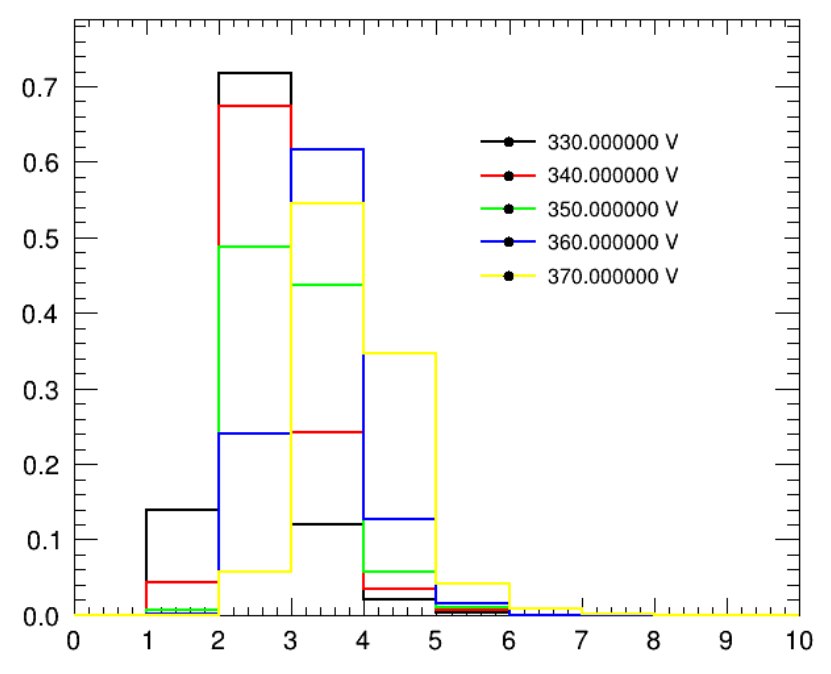
\includegraphics[width=0.5\linewidth]{desy_mult}
  \caption{The number of pads in the cluster in the DESY test versus the MM voltage.}
  \label{fig:tpc:desy_mult}
\end{figure}

The dE/dx resolution and the collected charge for the different detector parameter scans are presented in \autoref{fig:tpc:desy_dedx1}---\ref{fig:tpc:desy_dedx4}.

\begin{figure}[!ht]
  \centering
  \begin{minipage}{0.49\linewidth}
    \centering
    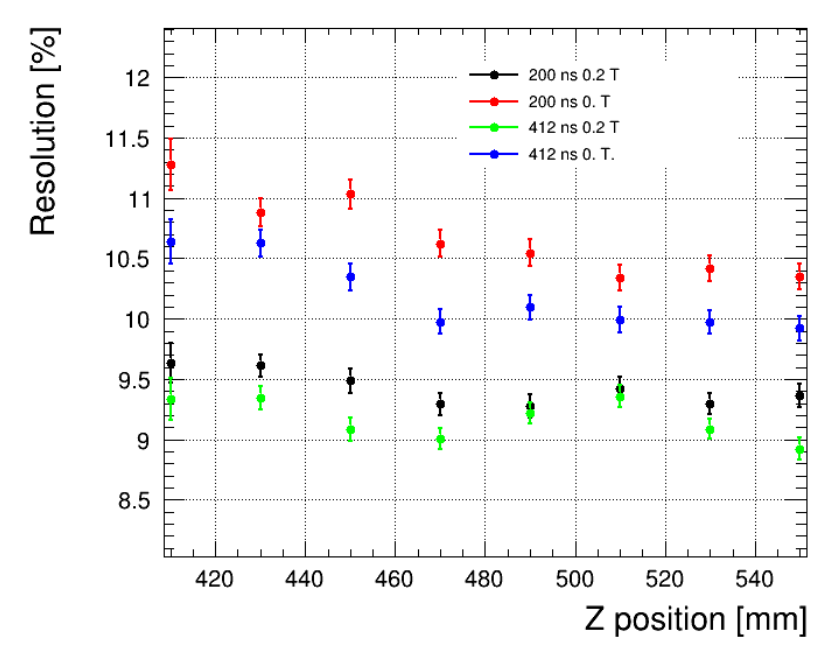
\includegraphics[width=0.8\linewidth]{desy_resol_pos} \\ (a)
  \end{minipage}
  \begin{minipage}{0.49\linewidth}
    \centering
    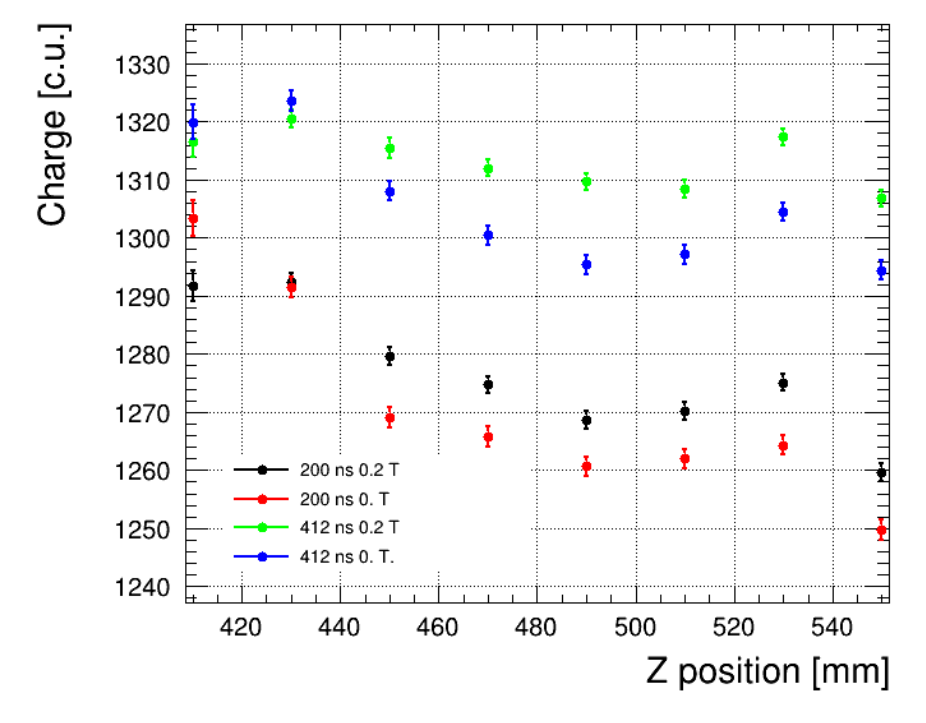
\includegraphics[width=0.8\linewidth]{desy_charge_position} \\ (b)
  \end{minipage}
  \caption{The dE/dx resolution (a) and average charge per cluster (b) for the 4 GeV/c electron tracks in the DESY beamtest versus the drift distance (a.u.) for different peaking time and magnetic field setup.}
  \label{fig:tpc:desy_dedx1}
\end{figure}

\begin{figure}[!ht]
  \centering
  \begin{minipage}{0.49\linewidth}
    \centering
    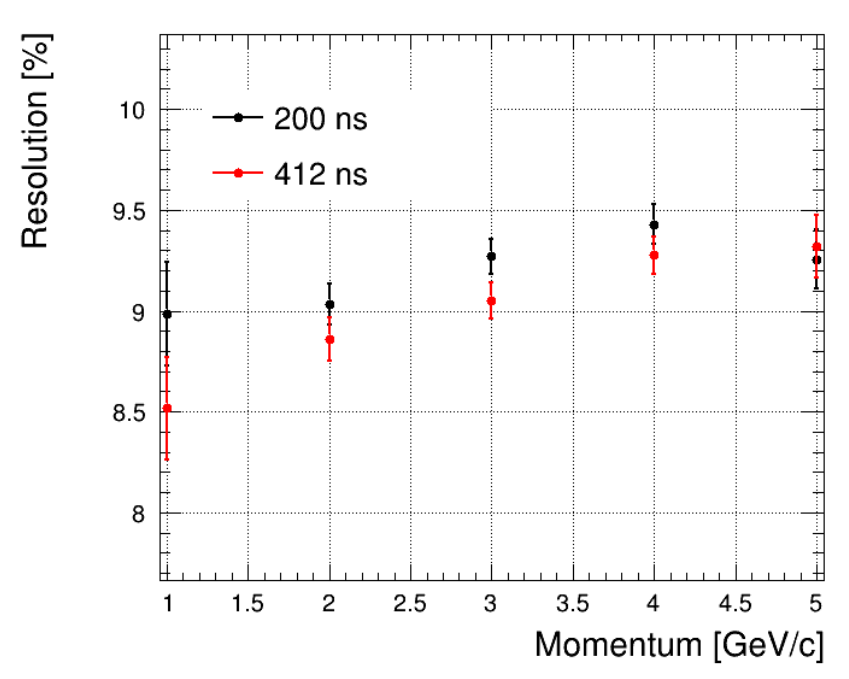
\includegraphics[width=0.8\linewidth]{desy_resol_mom} \\ (a)
  \end{minipage}
  \begin{minipage}{0.49\linewidth}
    \centering
    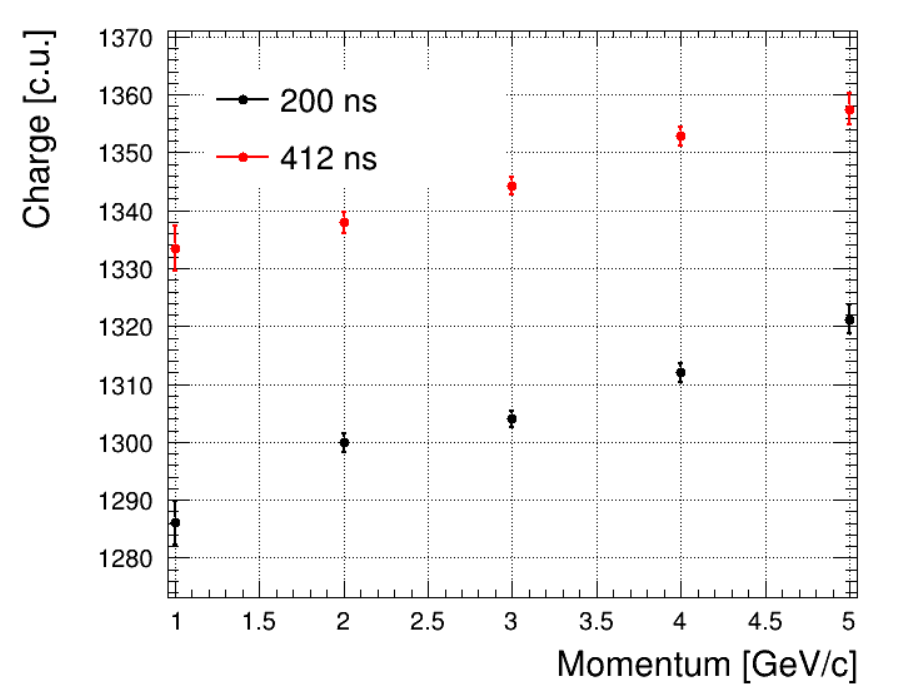
\includegraphics[width=0.8\linewidth]{desy_charge_mom} \\ (b)
  \end{minipage}
  \caption{The energy resolution (a) and average charge per cluster (b) for the electron tracks in the DESY beamtest versus the track momentum for different peaking time. The magnetic field is set to 0.2T, the track position is set to 430 mm along Z axis.}
  \label{fig:tpc:desy_dedx2}
\end{figure}

\begin{figure}[!ht]
  \centering
  \begin{minipage}{0.49\linewidth}
    \centering
    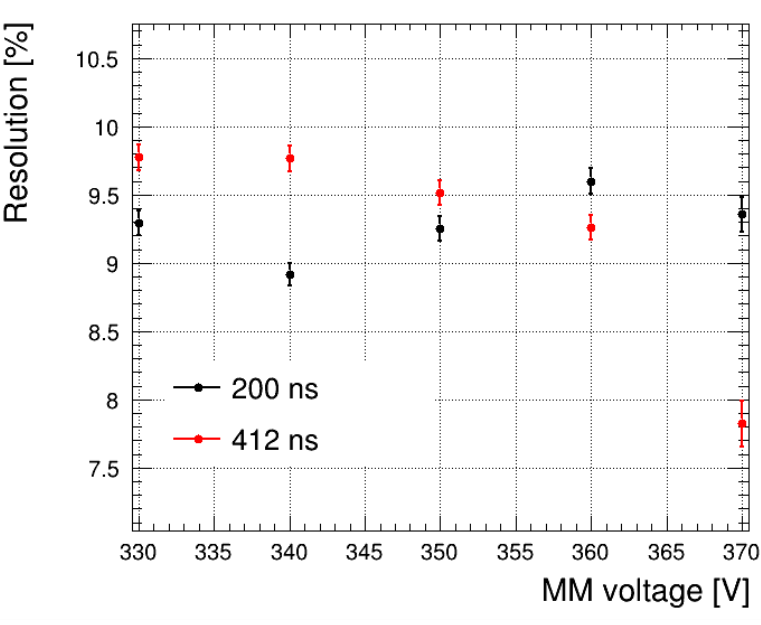
\includegraphics[width=0.8\linewidth]{desy_resol_hv} \\ (a)
  \end{minipage}
  \begin{minipage}{0.49\linewidth}
    \centering
    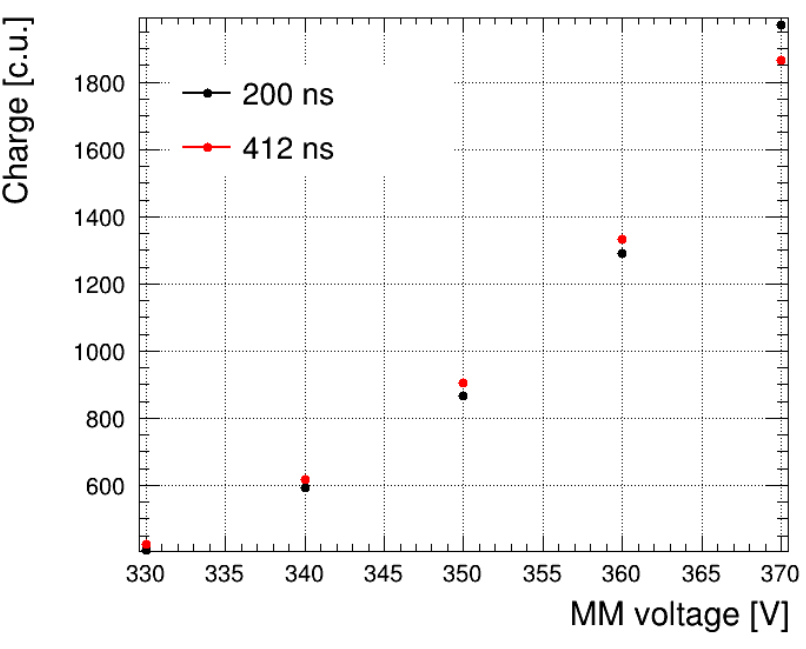
\includegraphics[width=0.8\linewidth]{desy_charge_hv} \\ (b)
  \end{minipage}
  \caption{The energy resolution (a) and average charge per cluster (b) for the 4 GeV/c electron tracks in the DESY beamtest versus the Micromegas voltage for different peaking time. The magnetic field is set to 0.2T, the track position is set to 430 mm along Z axis.}
  \label{fig:tpc:desy_dedx3}
\end{figure}

\begin{figure}[!ht]
  \centering
  \begin{minipage}{0.49\linewidth}
    \centering
    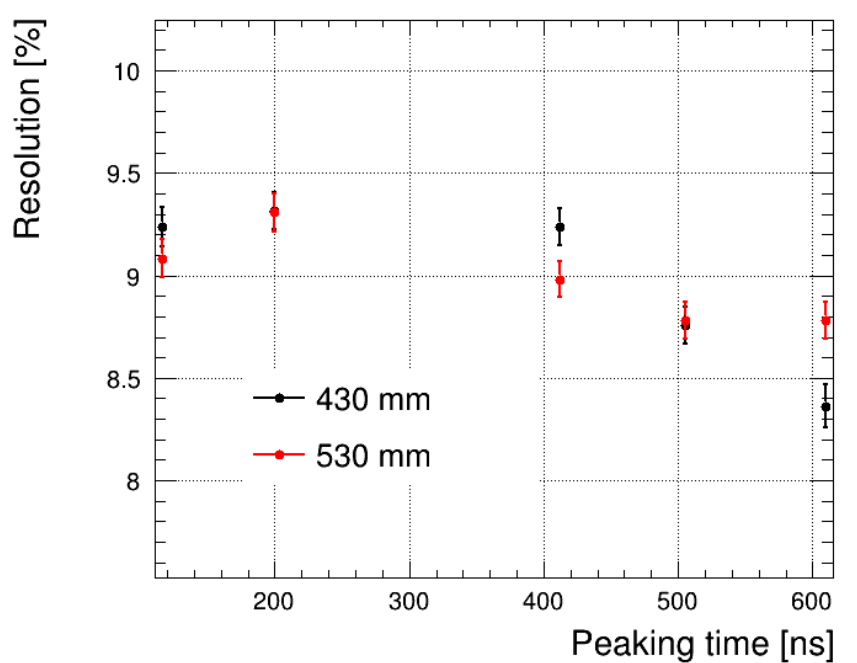
\includegraphics[width=0.8\linewidth]{desy_resol_peaking} \\ (a)
  \end{minipage}
  \begin{minipage}{0.49\linewidth}
    \centering
    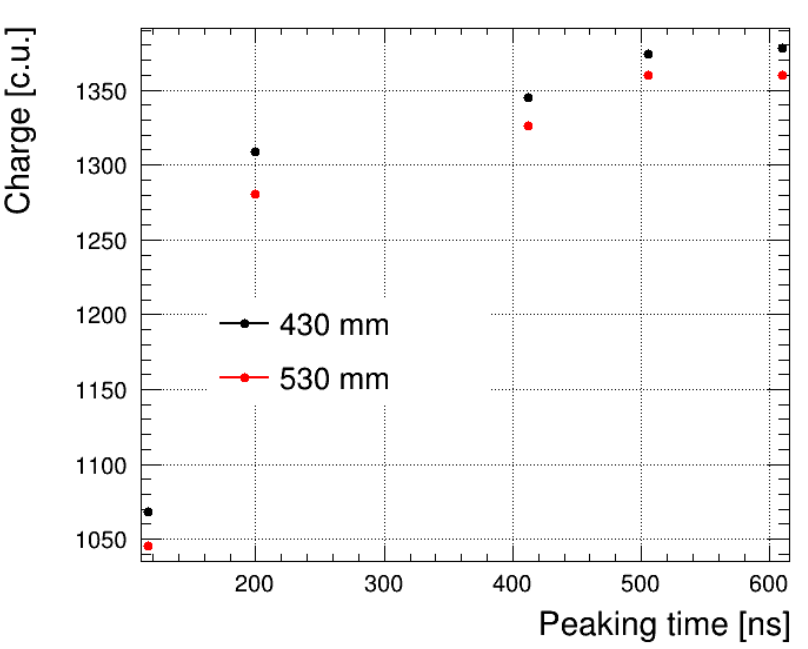
\includegraphics[width=0.8\linewidth]{desy_charge_peaking} \\ (b)
  \end{minipage}
  \caption{The energy resolution (a) and average charge per cluster (b) for the 4 GeV/c electron tracks in the DESY beamtest versus the peaking time for different drift distances (a.u.). The magnetic field is set to 0.2T.}
  \label{fig:tpc:desy_dedx4}
\end{figure}

From these plots, we can see that the resolution remains stable over the different parameters of the setup. Though I found some expected dependencies. The presence of the magnetic field improves the charge collection and also improves the energy resolution (\autoref{fig:tpc:desy_dedx1}). The dependence of the resolution and the collected charge over the drift distance is not completely understood. The larger collected charge in the sample at 530 mm position is not expected as there is nothing specific in it. We suspect the electric field uniformity as a possible reason for such an effect.

Overall, the energy resolution was estimated below 10\% for nearly all the samples with the magnetic field. In the absence of the field the dE/dx resolution is below 12\%. As before, we are using one module so for the proper comparison with the existing TPCs performance, the result should be scaled with $1/\sqrt{2}$. It will give us 7\% resolution that is the same as what we observed in the existing ND280 TPCs.

\subsubsection{Spatial resolution}
The PRF technique described in the CERN test section was used to estimate the spatial resolution of the new setup. The various scans with horizontal tracks were used to evaluate the dependence of the resolution over the detector parameters. The result is shown in \autoref{fig:tpc:sr1} and \autoref{fig:tpc:sr2}. The spatial resolution below 220 $\mu$m was observed over all drift distance region. It was found that the higher voltage provides remarkable improvements in the detector performance decreasing the resolution from 300 $\mu$m down to 150 $\mu$m. The higher voltage cause the larger amplification. Therefore more pads detect the signal with the charge spreading. With more pads the more robust position extraction is possible. It was also found that the peaking time has no strong influence of the resolution that allows to choose any value of this parameter.

\begin{figure}[!ht]
  \centering
  \begin{minipage}{0.49\linewidth}
    \centering
    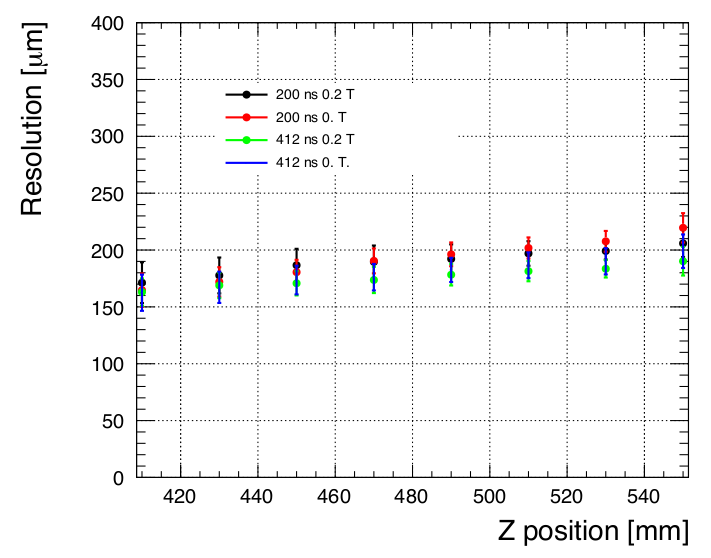
\includegraphics[width=0.8\linewidth]{desy_sr_pos} \\ (a)
  \end{minipage}
  \begin{minipage}{0.49\linewidth}
    \centering
    \includegraphics[width=0.8\linewidth]{desy_sr_hv} \\ (b)
  \end{minipage}
  \caption{The spatial resolution of the DESY test versus the drift distances (a.u.) (a) and the Micromegas voltage (b)}
  \label{fig:tpc:sr1}
\end{figure}

\begin{figure}[!ht]
  \centering
  \begin{minipage}{0.49\linewidth}
    \centering
    \includegraphics[width=0.8\linewidth]{desy_sr_mom} \\ (a)
  \end{minipage}
  \begin{minipage}{0.49\linewidth}
    \centering
    \includegraphics[width=0.8\linewidth]{desy_sr_peaking} \\ (b)
  \end{minipage}
  \caption{The spatial resolution of the DESY test versus the track momentum (a) and the peaking time (b)}
  \label{fig:tpc:sr2}
\end{figure}

The electron beam in the facility is spread in space. The beam profile can be described with a Gaussian shape with a sigma around 1 cm. This allows us to study the dependence of the spatial resolution from the track position in the pad. The detector is kept at the same position but because of the natural beam spread tracks cross pads in the different positions. The obtained spatial resolution versus the position in the pad is shown in \autoref{fig:tpc:sr_pad}. I observed a significant variation of the resolution. It changes from 100 $\mu\text{m}$ at the pad border up to 200 $\mu\text{m}$ in the pad center. The behavior is mostly understood. When a track crosses a pad center the pad multiplicity in the perpendicular direction is lower compared to the case when the track goes over the border of two pads. More pads detect the signal more accurate position reconstruction in the cluster we expect. The effect can be reduced with implementation of larger charge spreading. But the tracking in case of events with many particles will be more difficult. The investigation of the possible analyses algorithm improvements is ongoing. The Mont--Carlo simulation can help with testing the different detector configurations and obtaining the best one. The MC algorithm is under development, we are looking for the best analytical description of the charge sharing effect. Since the simulation toolkit is established, we can test various detector configuration with different reconstruction algorithms to find the best combination.

\begin{figure}[!ht]
  \centering
  \includegraphics[width=0.6\linewidth]{desy_sr_pads}
  \caption{The spatial resolution versus the track position in the pad in the particular column. The pad borders are represented with the vertical lines.}
  \label{fig:tpc:sr_pad}
\end{figure}

\subsubsection{DESY test results}
The DESY test analyses has already demonstrated the large improvement of the spatial resolution. Values below 200 $\mu\text{m}$ were reached. The energy resolution was observed at the level of the existing ND280 TPCs.

The analyses of the beamtest data is still ongoing. Many improvements can be made. For example, we are working on a better understanding of the waveforms that will allow us to get rid of taking the maximum amplitude but use the information from the whole distribution. For this a good understanding of the electronics is required. The possible benefit is a more precise treatment of the charge in a pad resulting in better spatial resolution. A precise description of the detector response will also help a lot with the future Monte--Carlo simulations. In the T2K the MC simulation is an integral part of the analyses. A good detector model is required for future HA--TPC.

The other major improvement that can be made is the development of a different algorithm for track reconstruction. The PRF method demonstrated good performance for the horizontal tracks, but it looses the precision for the inclined tracks. Better analyses techniques are under investigation.

\section{Conclusion}
The high angle TPCs will play an important role in the upgraded near detector of the T2K experiment. The new field cage and the new MicroMegas detector with the resistive foil were designed. The prototypes of the TPC with the resistive anodes were tested in the different regimes. I found that the energy resolution will not be worse compared to the existing TPCs, which is critical for the $\nu_e$ measurements in T2K. The spatial resolution will be improved that will provide more precise momentum reconstruction.

As was mentioned in the introduction the improved spatial resolution will not gain the neutrino energy reconstruction accuracy under the CCQE reaction assumption. The smearing effect of the Fermi motion is larger than the uncertainty on the lepton momentum. But some analyses can improve the accuracy with more precise momentum reconstruction. T2K spent a lot of effort on studying nuclear effects such as Fermi motion, FSI, nucleon correlation effects. It is already the dominant systematic on current T2K measurements of oscillation parameters and will soon become the principal precision limitation. There are plenty of models describing the effects, but the precision of the measurements does not allow us to select the most appropriate one. In our experiment, to study the nuclear effects, we use the kinematic imbalance between the final state lepton and hadrons in the plane transverse to the neutrino direction~\cite{Lu2016}. The presence of such an imbalance explicitly indicates the nuclear effects.
This particular approach allows studying the effects of interest with minimal dependence from the incoming neutrino energy. Also, it provides the natural separation between Fermi motion effects and nucleon correlation. This is very helpful in the determination of the appropriate model. As we can study the kinematic region where Fermi motion is severely suppressed this effect will not provide the domination smearing anymore. Thus the improvements in the momentum resolution will gain the physics analyses performance. One more analyses technique that will be able to improve its performance with the new TPCs is an analysis of the pion production in a neutrino interaction. The double transversal momentum imbalance is a technique~\cite{Lu2015} that can distinguish the neutrino interactions with Hydrogen and Carbon in our scintillator target. Such an analysis will also gain performance with more precise momentum measurements. This list of possible improvements is not limited to the studies mentioned above. Any analysis that requires the momentum precision better than 10\% will gain accuracy with the new detectors.

The production of the HA--TPC is ongoing and the installation is planned for 2022.


\end{document}